% 导言区
\documentclass[12pt]{article} %article book report letter

\usepackage{ctex}
\usepackage{graphicx}
\usepackage{amsmath}
\usepackage{amssymb}
\usepackage{geometry}
\usepackage{graphicx}

\usepackage{float}

%\usepackage[super]{gbt7714}
\usepackage{xcolor}

\usepackage{verbatim}

%\usepackage{natbib}
%\setcitestyle{authoryear,round}

%\usepackage[numbers, sort&compress]{natbib}
\usepackage{gbt7714}
\bibliographystyle{gbt7714-numerical}
%\usepackage[backend=biber,style=gb7714-2015ay]{biblatex}
%\usepackage[backend=biber,style=gb7714-2015ay,gbnoauthor=true]{biblatex}

\usepackage{hyperref}

\geometry{top=3cm,bottom=3cm}

\hypersetup{hidelinks,
	colorlinks=true,
	allcolors=black,
	pdfstartview=Fit,
	breaklinks=true
}

\usepackage{listings,lstautogobble}

%\usepackage{listings} 
\usepackage{xcolor}

%\usepackage{minted}


\begin{document}
	\thispagestyle{empty}
	\begin{figure}[ht]
		\centering
		
\includegraphics[scale=0.56]{SYSULogo.pdf}
	\end{figure}
	
	\begin{center}
		\textbf{{\fontsize{35pt}{0pt}本科生毕业论文 (设计)}}
		
		\Large \textbf{{\fontsize{25pt}{0pt}Undergraduate Graduation Thesis (Design)}}
	\end{center}
	
	\begin{center}
		\huge 题目:\textbf{\underline{中国A股市场定价因子选择}}
		
		\textbf{\underline{与股价收益率预测}}
	\end{center}
	
	\begin{quotation}
		\large \noindent
		院系 \\
		School(Department):\underline{~~~~~~~~~~~~~~~~~~数学学院~~~~~~~~~~~~~~~~~~~} \\
		专业 \\
		Major:\underline{~~~~~~~~~~~~~~~~~~~~~~~~~~~~~~~~数学与应用数学~~~~~~~~~~~~~~~~} \\
		学生姓名 \\
		Student Name:\underline{~~~~~~~~~~~~~~~~~~~~~~~~~~张景桐~~~~~~~~~~~~~~~~~~~~~~} \\
		学号 \\
		Student No:\underline{~~~~~~~~~~~~~~~~~~~~~~~~~~~~18315133~~~~~~~~~~~~~~~~~~~~~} \\
		指导教师(职称) \\
		Supervisor(Title):\underline{~~~~~~~~~~~~~~~~~刘立新~~教授~~~~~~~~~~~~~~~~~~~}
	\end{quotation}
	~\\
	\begin{center}
		时间:二零二二年四月十一日
		
		Date: April 11th 2022
	\end{center}
	
	\newpage
	\thispagestyle{empty}
	\begin{center}
		\Large  学术诚信声明
	\end{center}
	
	\begin{large}
	本人所呈交的毕业论文,是在导师的指导下,独立进行研究 工作所取得的成果,所有数据、图片资料均真实可靠。除文中已经注明引用的内容外,本论文不包含任何其他人或集体已经发表或撰写过的作品或成果。对本论文的研究作出重要贡献的个人和集体,均已在文中以明确的方式标明。本毕业论文的知识产权归属于培养单位。本人完全意识到本声明的法律结果由本人承担。\\ \\ \\
	$~~~~~~~~~~~$本人签名:$~~~~~~~~~~~~~~~~~~~~~~~~~~~~~~~$日期:
	\end{large}
	~\\ \\ \\
	\begin{center}
		\Large \textbf{Statement of Academic Integrity}
	\end{center}

	\begin{large}
	I hereby acknowledge that the thesis submitted is a product of my own independent research under the supervision of my supervisor, and that all the data, statistics, pictures and materials are reliable and trust- worthy, and that all the previous research and sources are appropriately marked in the thesis, and that the intellectual property of the thesis be- longs to the school. I am fully aware of the legal effect of this statement. \\ \\ \\
	$~~~~~~~~$Student Signature:$~~~~~~~~~~~~~~~~~~~~~~~~~~$Date:
	\end{large}
	\newpage
	\thispagestyle{empty}
	\begin{center}
		\LARGE \textbf{中国A股市场定价因子选取与股价收益率预测}
		%\LARGE \textbf{基于变量因子选择的中国 A 股市场量化交易研究}
	\end{center}
	\begin{center}
		\textbf{摘要}
	\end{center}
	
	%本文对中国A股市场量化交易进行分析,根据中国A股市场的股票定价因子对股价收益率进行预测。首先,在众多的定价因子进行选择,即特征选取和变量选取,目的是选择互相正交且重要的定价因子,对自变量进行降维,减少信息冗余,提高后续预测模型的训练精度;其次,将选取的特征作为输入,通过机器学习算法,比如常见的随机森林和神经网络等算法对下一期的股价进行预测;最后,根据预测的收益率,做多收益率最高的10\%的股票,做空收益率最低的10\%的股票,构造一个多空头寸的投资组合,对投资组合的收益率和夏普比率进行分析。
	
	本文选取了1998-2018年的中国A股市场数据对中国A股市场的量化交易进行研究。本文首先介绍了贝叶斯变量选择的思想与原理,然后根据贝叶斯变量选择方法对中国A股市场中的定价因子进行选择,寻找出对股价收益率有驱动作用的因子,其中发现收益率波动率、最大日收益率、交易额波动率和账面市值比等因子对股价收益率影响较大,这一结果与LASSO算法得到的结果相近似。然后,本文选取了两种典型的预测算法,一种是线性回归方法,另一种是能较好捕抓数据非线性结构的XGboost树方法。我们利用预测算法对股价收益率进行预测,做多预测收益率最高10\%的股票,做空预测收益率最低10\%的股票,构造出一个投资组合。线性回归方法构造的投资组合年化收益率约为31.5\%,夏普比率为1.78,XGboost算法的年化收益率为38.8\%,夏普比率为2.2,相较于简单的市场组合策略,收益率和夏普比率都得到显著提升。最后,我们发现通过利用选择出的部分定价因子变量来进行模型训练,在能够减少训练时间的同时,并可以得到与用全部变量来训练模型相近的效果。
	
	\textbf{关键词:变量选择~  机器学习~预测}
	
	\newpage
	\thispagestyle{empty}
	\begin{center}
		\large \textbf{Pricing Factor Selection and Stock Return Prediction in Chinese Stock Market} ~\\ ~\\
		\normalsize \textbf{Abstract}
	\end{center}
	
	This paper uses data of China's A-share market from 1998 to 2018 to study the quantitative trading in Chinese A-share market. Firstly, we introduce the method of Bayesian variable selection, and then selects the important pricing factors in China's A-share market, which drive the stock price return. We find that the factors such as return volatility, maximum daily return, trading volume volatility and book to market value ratio have a great impact on the stock price return. This result is similar to that obtained by lasso algorithm. Secondly, we select two typical prediction algorithms, one is linear regression method, the other is xgboost tree method which can better capture the nonlinear structure of data. We use these prediction algorithms to predict the stock price return. We long the stocks with the highest 10 \% predicted return, short the stocks with the lowest 10 \% predicted return, and construct a portfolio. The annual return and Sharpe ratio of portfolio constucted by linear regression are 31.5\% and 1.78. Similarly, the annual return and Sharpe ratio of portfolio constucted by XGboost are 38.8\% and 2.2. Compared to market portfolio, the portfolios constructed by linear regression and XGboost have much better performance in both annual return and Sharpe ratio. Finally, we find that by using the selected pricing factor variables to train the model, we can reduce the training time and get the similar effect with all variables.
	
	\textbf{Key words: Variable Selection~ Machine Learning~ Prediction}
	
	\newpage
	\thispagestyle{empty}
	\tableofcontents
	
	\newpage
	\thispagestyle{empty}
	\listoffigures
	
	\listoftables
	
	\newpage
	\setcounter{page}{1}
	\section{引言}
	
	\subsection{选题背景与意义}
	在金融资产定价领域中,许多实证研究目前已经找到了许多驱动股票收益率变化的因子。金融领域中的因子也称因素,相当于预测模型中的自变量,而股票的收益率则相当于模型中的因变量,通过因子可以对股票价格进行预测,
	常见的预测方法包括线性模型,随机森林和神经网络等方法。在对下一期股价收益率进行预测之后,可以选择做多预测收益率最高的10\%的股票,即购买收益率最高的股票,并且做空收益率最低的10\%的股票,即向券商部门借入股票,然后在当期卖出这些股票,下一期等股票价格下跌,再买入还给券商部门,通过做多和做空两种方法以此构造一个多空头寸的投资组合。
	目前对冲基金在进行量化投资交易时主要依赖于两步法对资产进行管理,第一步是通过变量因子估计未来股票的收益率,在预测中的关键是输入变量的选取构造,以及预测方法的应用,然后第二步再根据预测收益率对资产进行组合优化,构造一个投资组合以最大化收益率或夏普比例等目标\cite{cong2021alphaportfolio},因此收益率预测是金融中一个重要的问题。
	
	如今,金融学术论文中已经找到了超过400多个与股票收益率有关的定价因子,多数因子具有明确的经济含义,可以对其经济因果含义进行合理解释,比如账面市值比高的公司股票,一般成长潜力较大,更加容易产生较高的收益率。但是由于发表导向使得金融学术界掀起了挖掘因子的狂热浪潮,在这些发现得到的因子中许多可能具有较强的相关性,并非是独立的,比如季节因子和时间动量因子,存在一定关联关系,相关系数为0.63,自变量相关性在线性模型中给统计推断带来了很大干扰,甚至一些因子是数据窥探而得到的产物\cite{feng2020taming}。挖掘因子的浮躁态度也引起了许多学者的警惕,2011年John Cochrane在美国金融协会主席演讲时用“因子动物园” (factor zoo) 一词来描述金融学术界因子研究的现状,并提出了两个重要的问题:(1)哪些因子是独立正交的?(2)哪些因子是重要的?同时高维度的因子(即模型中的自变量)也给统计推断带来了许多问题,计量经济学中常根据线性回归中的系数判断自变量和因变量之间的相关性,当时当变量维度过高,而样本数量太少时候,会对系数估计结果产生较大的误差影响,所以在研究当中有必要找出重要且独立的因子,对模型进行降维处理,常用的方法有LASSO和贝叶斯方法等。
	
	因此本文的研究问题主要有如下两个,第一个问题是在中国股票市场的众多因子中寻找出独立且重要的股票定价因子,在线性模型中根据贝叶斯方法对模型的自变量重要性进行诊断,主要使用参考统计四大期刊中Mitchell和Beauchamp(1988)提出的方法\cite{mitchell1988bayesian},寻找出重要因子后可以对模型进行了降维效果,可以减少自变量中的信息冗余,提高输入特征的信噪比,并且加快后续模型的训练速度。第二个问题是根据找到的重要因子对股票价格收益率进行预测,使用到的方法包括线性回归方法以及能够较好捕抓数据非线性结构的XGboost方法,进而构造投资组合,并通过实际数据对方法进行回测,评价该策略的收益和风险状况。
	
	%本文希望通过数学手段在中国市场回答第一个和第二个问题,找出对驱动股价收益率具有重要意义的因子。站在数学研究的角度而言,这相当于是对模型变量进行选择,尝试着对模型进行优化。对高维模型的变量进行简化,一方面可以降低模型维度,提高模型训练速度,另一方面,可以剥离相关性较强的变量,减少变量中信息冗余,提高输入特征的信噪比,通过数学模型和经济解释对股价驱动因子进行检验,对中国实际A股市场交易具有重要意义,在统计研究中与此类似的问题也有利用变量选择技术提取与药物反映相关的重要影响因子,并对药物的反映做预测。
	
	%在选择出对股票价格具有重要驱动力的因子后,我们通过这些因子对股票价格收益率进行预测常见的投资组合构造方法有多空头寸对冲方法,以及马科维茨优化方法\cite{markowitz1952utility}。并通过实际数据对方法进行回测,评价该策略的收益和风险状况。
	
	\subsection{国内外研究现状和相关工作}
	
	在国内金融学研究中,在传统的Fama-French线性三因子的模型上,许多研究者根据中国金融市场规律,发现了许多对股价具有驱动力的因子。苏冬蔚和麦元勋(2004)通过实证检验发现我国股市存在显著的流动性溢价,换手率低、交易成本高且流动性小的资产具有较高的预期收益,产生流动性溢价的原因是交易成本而不是交易频率\cite{苏冬蔚2004流动性与资产定价}。田利辉等(2014)发现我国股市收益率反转的特征,构造了反转因子\cite{田利辉2014反转效应与资产定价},而林建浩等(2021)基于结构向量自回归模型和随机波动率模型测度货币政策不确定性,发现货币政策不确定性是中国股票市场收益率的重要定价因子\cite{林建浩2021货币政策不确定性是中国股票市场的定价因子吗}。关于中国股票市场上的因子研究,还有许多的探讨,同时也存在许多文献根据定价因子和股票基本面特征利用机器学习方法搭建量化交易策略。李斌等(2019)认为基本面量化投资是近年来金融科技和量化投资研究的新热点,并利用96种因子,通过预测组合算法、Lasso回归、岭回归和神经网络等12种机器学习算法构建股票收益预测模型及投资组合,发现深度前馈网络在筛选因子数据上的多空组合月度收益达到了3.41\%,年化收益率约为40.8\%,比传统线性算法要更好\cite{李斌2019机器学习驱动的基本面量化投资研究}。Leippold等(2021)同样采用机器学习算法框架,但在构造输入特征时,结合宏观经济变量和90个因子的张量乘积和行业变量作为输入特征,能对机器学习的性能进行改善,在2013-2020年的回测周期中,投资组合的收益率也大幅度提升,通过XGboost算法得到的年化收益率约为37\%,夏普比率为1.67,神经网络算法得到的年化收益率为60\%,夏普比率约为3\cite{leippold2021machine}。在国外的研究当中,Shihao Gu等(2020)在美国股票市场使用机器学习算法对月频因子数据进行分析构造投资组合也得到较好的效果\cite{gu2020empirical}。
	
	因子投资是资产定价领域的重要部分,然而关于选择出具有对股票有驱动力的因子一直也存在争议。许多学者们通过贝叶斯方法对模型进行诊断分析,寻找出对驱动股票收益率具有实质意义的因子,并且最优化投资组合的夏普比率\cite{anderson2016robust}。Barillas和Shanken(2018)对先验概率进行拓展,根据线性模型中因子在时间序列中的表现找出重要的定价因子\cite{barillas2018comparing}。Bryzgalova等(2019)通过贝叶斯方法对线性的资产定价模型进行分析,提出了简单且稳定的寻找重要因子框架,能够分辨出模型中不可替代和可替代的因子\cite{bryzgalova2019bayesian}。Feng等(2020)结合LASSO算法构造两步的正则化回归来对新的因子有效性进行检验,并对由于遗漏变量导致的模型选择偏差做出解释\cite{feng2020taming}。Kozak等(2020)通过主成分分析等方式对因子进行降维,并比较因子对股票收益率的样本外预测效果\cite{kozak2020shrinking}。
	
	同时Guyon和Elisseeff(2003)总结了变量选择的三个作用,第一可以提高预测性能,第二可以加快训练速度并选择出更有效的预测因子,第三可以对模型有更强的解释力\cite{guyon2003introduction}。
	
	本文研究目的是通过量化投资的方法在中国A股市场中设计出有效的交易策略,设计出优化投资组合收益率和夏普比率的方案,并对中国A股市场中的定价因子进行讨论,给中国A股市场量化投资带来启示。首先通过数学与统计原理并结合参考文献,对中国市场中股票收益率的定价因子有效性与模型选择进行探讨,尝试着对已有的变量因子选择理论进行改进,然后根据得到预测模型和输入特征变量对股票收益率进行预测,并根据构造投资组合。
	
	\subsection{本文论文结构与章节安排}
	本文共分为五节,每章节的内容如下:
	
	第一节:引言。
	
	第二节:数据描述,对使用的数据与变量因子进行描述,并进行数据预处理。
	
	第三节:定价因子变量选择,使用贝叶斯变量选择方法对股票收益率的定价因子进行检验,找出中国市场上对股票价格有驱动意义的定价因子。
	
	第四节:股票收益率预测,根据选取的因子变量和预测模型对股价收益率进行预测,并构造投资组合,进行回测分析投资组合的收益率和夏普比率,并分析程序运行的时间。
	
	第五节:总结与展望,对文章中的工作进行总结,并提出未来的研究展望。

	\newpage
	\section{数据描述}
	\subsection{数据来源}
	本文选取1998年-2018年中国A股市场中的股票进行研究,时间频度为月度频率。数据来源分为两部分,一部分是来源于CSMAR数据库,CSMAR数据库是中国公司财务信息最全的数据库,其中选取的财务数据与公司的比率结构,偿债能力和发展能力有关,包括流动资产比率等19项指标,另一部分则是从李斌等(2018)整理公开的中国定价因子数据中获取,其中包括收益率波动率等15项指标指标\cite{李斌2019机器学习驱动的基本面量化投资研究},因此所有定价因子即自变量的维度为35维,具体使用的定价因子可以在附录中找到。初始选取的股票为A股市场的所有股票,与文献中常见的处理方法类似,由于ST股票存在退市风险,会成为极端值影响研究,所有将其剔除掉,另外金融行业与其他行业有别,基本面数据存在较大的差异,因此分析的股票中也不考虑金融行业的公司,同时避免单只股票训练样本太少的问题,因此要求股票至少要上市一年才纳入样本当中。
	
	
	\subsection{数据处理}
	在使用数据前,数据进行预处理工作。首先是对缺失值进行处理,对于公司资产负债表数据,此类财务披露频度为季度,对于缺失值的处理为采用上一期披露的数据,若之前该项指标一直没有数据记录,则以0来代替。其次是数据标准化工作,标准化可以使得训练时能够得到更好的效果,本文采用正态标准化对数据进行处理
	$$x^{\prime}=\dfrac{x-mean(x)}{std(x)}$$
	即通过正态转换将数据进行标准化处理,在训练模型的过程中,我们采用的是滚动期为12个月的训练方法。股票特征即定价因子为输入特征,对股票价格进行预测。机器学习方法都需要对模型中的参数进行训练,比如线性回归中参数。这里我们采用12个月周期的滚动期来对模型的参数进行训练。举例而言,当我们在预测2018年1月股价收益率的时候,我们的输入特征是2017年12月份股票的特征,这时我们需要对参数进行训练,我们利用的是2017年1至12月的股价收益率,以及2016年12月与2017年1至11月的股票特征来对模型进行训练,通过以往这12个月的数据来拟合出模型的参数,进而用于预测,在每个训练窗口中,我们对数据进行标准化以得到更好的训练效果。
	
	
	
	\newpage
	\section{定价因子变量选择 \label{S3}}
	
	在本节中,我们首先在\ref{S3.1}节中基于Mitchell和Beauchamp的方法\cite{mitchell1988bayesian}对贝叶斯在线性回归模型中进行变量选择的思想原理进行介绍,接着我们通过R语言中的Spikeslab包\cite{ishwaran2010spikeslab}对实际数据进行分析,寻找出对股价收益率具有影响的定价因子,并且将贝叶斯方法筛选出的变量与LASSO方法进行比较。
	
	
	\subsection{贝叶斯变量选择方法 \label{S3.1}}
	Mitchell和Beauchamp(1988)最先将贝叶斯应用到线性回归的变量选择当中\cite{mitchell1988bayesian},并提出spikeslab分布,而后George和Mcculloch等人对该方法不断改进,并提出利用Gibbs抽样器等方法来优化变量选择速度\cite{george1993variable,ishwaran2005spike}。
	
	下面对Mitchell和Beauchamp提出的在线性模型中根据贝叶斯方法对变量进行选择的原理进行阐述\cite{mitchell1988bayesian},线性回归模型形式可以表示为\eqref{E3.1}。
	\begin{equation}
		\mathbf{y}=\mathbf{X} \boldsymbol{\beta} + \boldsymbol{ \varepsilon} \label{E3.1}
	\end{equation}
	矩阵$\mathbf{X}$的维度为$n\times k$维,$\boldsymbol{\beta} $为对应的参数向量,将向量形式展开可以写成
	\begin{equation*}
		y= \alpha + \beta_1 x_1 + \beta_2 x_2 + \beta_2 x_3 +...+\beta_k x_k + \varepsilon
	\end{equation*}
	在线性回归中进行变量选择则是要从所有自变量$x_1,x_2,...,x_k$中选出对$y$有影响的变量,我们假设$A_m$是对$\mathbf{y}$有影响的变量的下标集合
	\begin{equation}
		p(A_m \mid \mathbf{y})=\dfrac{p(\mathbf{y} \mid A_m) \times p(A_m)}{p(\mathbf{y})} \label{EBB2}
	\end{equation}
	\eqref{EBB2}式中$p(A_m \mid \mathbf{y})$表达的含义则是我们在观测到数据$\mathbf{y}$的情况下,变量下标$A_m$其为真实模型的概率,这个式子可以通过贝叶斯公式的形式求出。
	
	
	相对于频率学派的观点,贝叶斯学派一般认为模型中的参数为随机变量,下面我们对模型参数$\varepsilon, \sigma^2$和$\boldsymbol{\beta}$的分布进行假设。
	
	我们首先假设$\varepsilon$服从均值为0,方差为$\sigma^2$的正态分布,并且$\varepsilon$之间相互独立。那么在给定$\boldsymbol{\beta}$和$\sigma^2$的情况下,$n$维向量$\mathbf{y}$应当服从均值为$\mathbf{X} \boldsymbol{\beta} $的正态分布,并且方差矩阵为$\sigma^2 \mathbf{I}$。然而在贝叶斯分布中,参数$\boldsymbol{\beta}$和$\sigma^2$通常是随机变量。这里假设$\sigma$是标准的无信息先验概率,即$ln(\sigma)$在$-ln(\sigma_0)$和$ln(\sigma_0)$中服从均匀分布,其中$\sigma_0$是一个非常大的数。对于$\beta$之间相互独立,服从"spike and slab"的分布,Mitchell和Beauchamp(1988)提出该spikeslab分布的概率密度函数如图\ref{spikeslab}中(a)所示,即$\beta_j$在$-f_j$到$f_j$中均匀分布,除了在$x=0$处会有一定的概率密度聚集,下面用公式严格刻画spikeslab分布。
	
	\begin{figure}[ht]
		
		\centering
		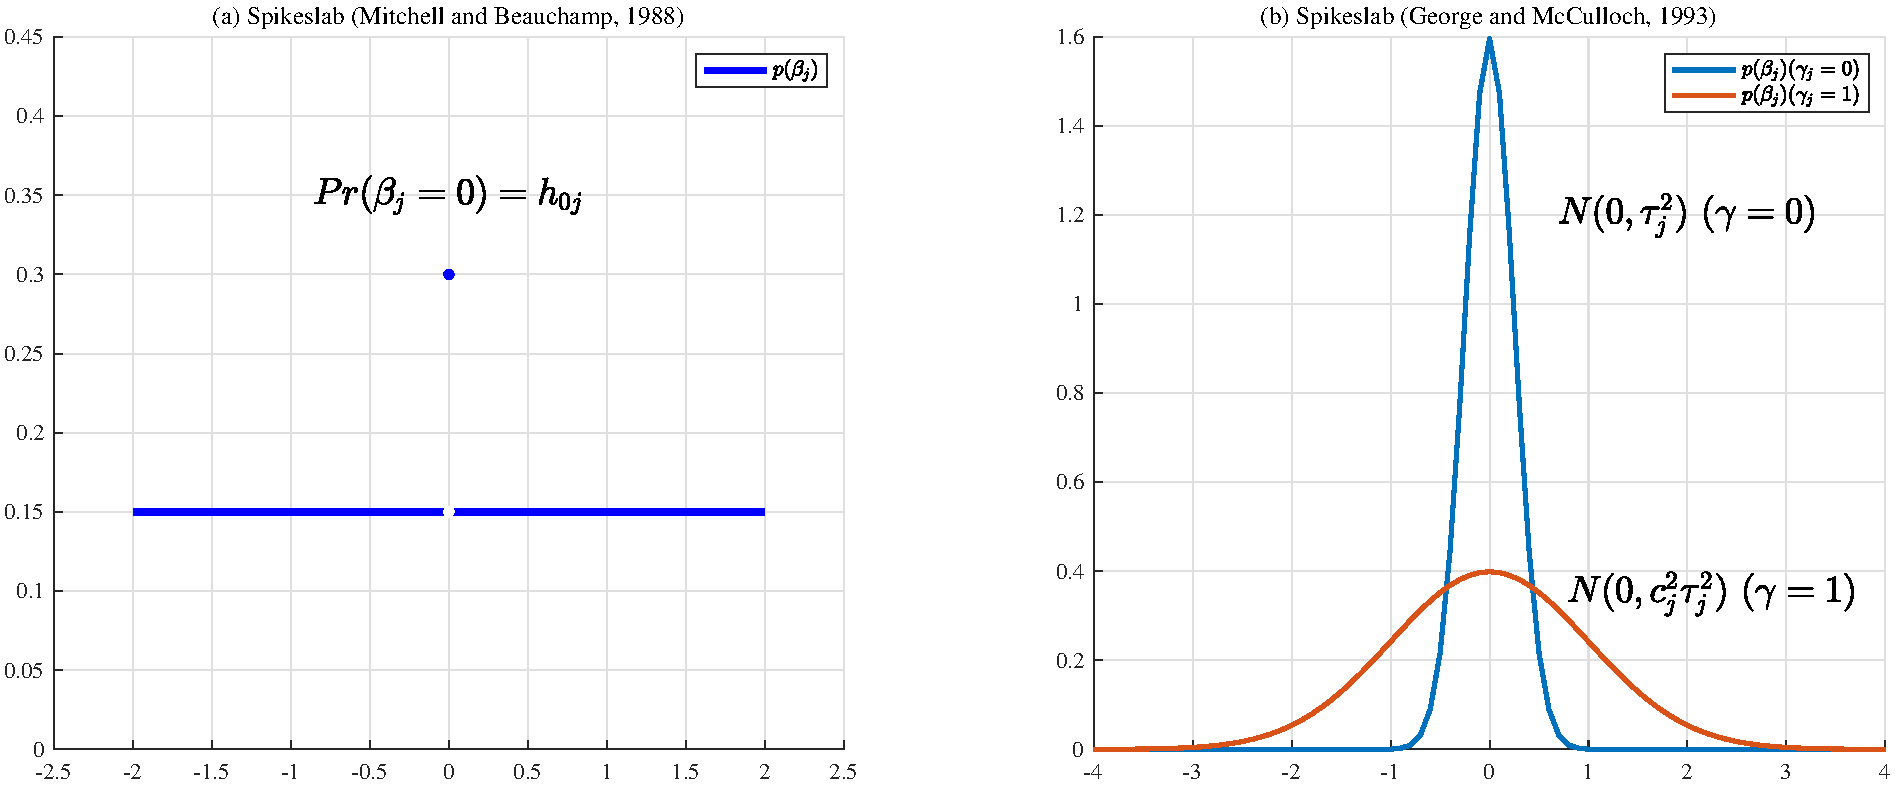
\includegraphics[scale=0.455]{spikeslab.pdf}
		\caption{spikeslab密度函数}
		\label{spikeslab}
	\end{figure}
	
	$\beta_j$的先验分布为spikeslab分布,可以表示为
	\begin{equation}
		\begin{gathered}
			\operatorname{Pr}\left(\beta_{j}=0\right)=h_{0 j} \\ \label{E3.4}
			\operatorname{Pr}\left(\beta_{j}<b, \beta_{j} \neq 0\right)=\left(b+f_{j}\right) h_{1 j}, \quad-f_{j}<b<f_{j}
		\end{gathered}
	\end{equation}
	即$\beta_j$的先验分布如图\ref{spikeslab}中(a)所示,在0点以外均匀分布,当$|\beta_j |>f_j$时概率为0
	\begin{equation}
		\operatorname{Pr}\left(\left|\beta_{j}\right|>f_{j}\right)=0
	\end{equation}
	其中$h_{0j}>0, h_{1j}>0$,且$h_{0j}+2h_{1j}f_j=1$。在该分布中,下式中的$\gamma_j$可以反应该分布的形状
	\begin{equation}
		\gamma_{j}=h_{0 j} / h_{1 j}=2 h_{0 j} f_{j} /\left(1-h_{0 j}\right) \label{E3.6}
	\end{equation}
	在\eqref{E3.6}中,$\gamma_j$表示尖顶(spike)高度除以厚块(slab)高度的比值。在上述概率分布下,子模型的先验分布为
	\begin{equation}
		\begin{aligned}
			\operatorname{Pr}\left(A_{m}\right) &=\prod_{\bar{J}_{m}} h_{0 j} \prod_{J_{m}}\left(2 f_{j} h_{1 j}\right) \\
			&=\prod_{\bar{J}_{m}} \gamma_{j} \prod_{J_{m}}\left(2 f_{j}\right) \prod_{j}\left(\gamma_{j}+2 f_{j}\right)^{-1} \label{E3.8}
		\end{aligned}
	\end{equation}
	\eqref{E3.8}可以理解在没有观测到$\mathbf{y}$时,从所有自变量$x_1,x_2,...x_k$中选择出下标为$A_m$自变量的概率。$\bar{J}_m$表示的是回归系数$\beta=0$的自变量下标集合,$J_m$则表示回归系数$\beta\neq 0$的自变量下标集合。结合之前的推导,自变量$\beta_j=0$的概率$Pr(\beta_j=0)$的概率为$h_{0j}$,不为0的概率则为$Pr(\beta_j \neq 0)=1-h_{0j}=2h_{1j}f_j$,\eqref{E3.8}则表示选择出$A_m$模型的概率,并且对应的自变量系数不为0.
	
	在对参数分布进行描述完后,我们开始计算\eqref{EBB2}所表示模型$A_m$的后验概率,即在观测到数据$\mathbf{y}$的情况下,$A_m$下标对应的自变量回归系数$\boldsymbol{\beta}$不为0的概率。
	
	在给定选取变量下标集合$A_m$,即自变量中只有$A_m$对应的自变量,其他自变量系数为0,从模型中剔除,并且再给定变量系数$\boldsymbol{\beta}_{m}$和$\sigma$后,变量$\mathbf{y}$的概率密度函数为
	\begin{equation}
		\begin{aligned}
			p(\mathbf{y} \mid A_{m}, \boldsymbol{\beta}_{m},\sigma)=(2 \pi)^{-n / 2} \sigma^{-n} \times \exp \left[- \dfrac{1}{2\sigma^2}(\mathbf{y}-\mathbf{X}_m \boldsymbol{\beta}_{m})^\prime(\mathbf{y}-\mathbf{X}_m \boldsymbol{\beta}_{m})\right] \label{Bayes2.8}
		\end{aligned}
	\end{equation}
	式子\eqref{Bayes2.8}的一项为
	\begin{equation*}
		\begin{aligned}
			(\mathbf{y}-\mathbf{X}_m \boldsymbol{\beta}_{m})^\prime(\mathbf{y}-\mathbf{X}_m \boldsymbol{\beta}_{m})&=(\mathbf{y}-\mathbf{X}_m\hat{\boldsymbol{\beta}}_{m}+\mathbf{X}_m\hat{\boldsymbol{\beta}}_{m}-\mathbf{X}_m \boldsymbol{\beta}_{m})^\prime(\mathbf{y}-\mathbf{X}_m\hat{\boldsymbol{\beta}}_{m}+\mathbf{X}_m\hat{\boldsymbol{\beta}}_{m}-\mathbf{X}_m \boldsymbol{\beta}_{m}) \\
			&=(\mathbf{y}-\mathbf{X}_m\hat{\boldsymbol{\beta}}_{m})^{\prime}(\mathbf{y}-\mathbf{X}_m\hat{\boldsymbol{\beta}}_{m})+ (\boldsymbol{\beta}_{m}-\hat{\boldsymbol{\beta}}_{m})^{\prime} \mathbf{X}_{m}^{\prime} \mathbf{X}_{m}(\boldsymbol{\beta}_{m}-\hat{\boldsymbol{\beta}}_{m}) \\
			&~~~+2(\mathbf{X}_m\hat{\boldsymbol{\beta}}_{m}-\mathbf{X}_m \boldsymbol{\beta}_{m})^\prime(\mathbf{y}-\mathbf{X}_m\hat{\boldsymbol{\beta}}_{m})
		\end{aligned}
	\end{equation*}
	并且由线性回归参数估计知识可以得到\eqref{E3.2}式
	
	\begin{equation}
		\hat{\boldsymbol{\beta}}_{m}=\left(\mathbf{X}_{m}^{\prime} \mathbf{X}_{m}\right)^{-1} \mathbf{X}_{m}^{\prime} \mathbf{y} \label{E3.2}
	\end{equation}
	即参数向量$\boldsymbol{\beta}$的估计$\hat{\boldsymbol{\beta}}$可以由\eqref{E3.2}给出
	,进而有$\mathbf{y}-\mathbf{X}_m\hat{\boldsymbol{\beta}}_{m}=0$,下式\eqref{E3.3}表示该线性模型的拟合优度。
	\begin{equation}
		S_{m}^{2}=\left(\mathbf{y}-\mathbf{X}_{m} \label{E3.3} \hat{\boldsymbol{\beta}}_{m}\right)^{\prime}\left(\mathbf{y}-\mathbf{X}_{m} \hat{\boldsymbol{\beta}}_{m}\right)
	\end{equation}
	结合式子\eqref{E3.3},故可将式子\eqref{Bayes2.8}写为下式\eqref{E3.9}
	\begin{equation}
		\begin{aligned}
			&p\left(\mathbf{y} \mid A_{m}, \boldsymbol{\beta}_{m}, \sigma\right)=(2 \pi)^{-n / 2} \sigma^{-n} \\
			&\quad \times \exp \left[-\frac{1}{2 \sigma^{2}}\left(S_{m}^{2}+\left(\boldsymbol{\beta}_{m}-\hat{\boldsymbol{\beta}}_{m}\right)^{\prime} \mathbf{X}_{m}^{\prime} \mathbf{X}_{m}\left(\boldsymbol{\beta}_{m}-\hat{\boldsymbol{\beta}}_{m}\right)\right)\right] \label{E3.9}
		\end{aligned}
	\end{equation}
	我们用\eqref{E3.9}乘以$p(\boldsymbol{\beta}_m \mid A_m,\sigma)$,其中$p(\boldsymbol{\beta}_m \mid A_m,\sigma)$可以理解为在知道模型真实模型$A_m$情况下,即在$A_m$对应的自变量系数不为0,而其他自变量系数为0,从模型中剔除时,所对应的$\boldsymbol{\beta}\neq 0$时的分布,故在概率为正的区域上有均匀分布$p(\boldsymbol{\beta}_m \mid A_m,\sigma)=\prod_{J_{m}}\left(2 f_{j}\right)^{-1} $。
	
	为了将$\boldsymbol{\beta}_m$消去,我们可以在\eqref{E3.9}乘以$p(\boldsymbol{\beta}_m \mid A_m,\sigma)$后对$\boldsymbol{\beta}_m$进行积分,注意这是一个多重积分,并且在被积函数中$\boldsymbol{\beta}_m$的形式类似于二次型,可以得到
	
	\begin{equation}
		\begin{aligned}
			&p\left(\mathbf{y} \mid A_{m}, \sigma\right)=\left(\prod_{J_{m}}\left(2 f_{j}\right)^{-1}\right) \\
			&\times(2 \pi)^{-\left(n-k_{m}\right) / 2}\left|\mathbf{X}_{m}^{\prime} \mathbf{X}_{m}\right|^{-1 / 2} \sigma^{-\left(n-k_{m}\right)} \exp \left[-S_{m}^{2} /\left(2 \sigma^{2}\right)\right] \label{E2.9}
		\end{aligned}
	\end{equation}
	其中$k_m$表示的是子模型$\mathbf{A}_m$中项的数目,在获得\eqref{E2.9}的过程中,我们假设$f_m$是足够大的,因此可以将积分区间从$(-f_j,f_j)$变换成$(-\infty,\infty)$\cite{mitchell1988bayesian}。然后再将\eqref{E2.9}乘以$p(\sigma \mid A_m)$,然后对$\sigma$进行积分可以得到
	\begin{equation}
		\begin{aligned}
			&p\left(\mathbf{y} \mid A_{m}\right)=\left(2 \ln \left(\sigma_{0}\right)\right)^{-1}\left(\prod_{J_{m}}\left(2 f_{j}\right)^{-1}\right) \pi^{-\left(n-k_{m}\right) / 2} \\
			&\quad \times\left(\frac{1}{2}\right) \Gamma\left(\frac{n-k_{m}}{2}\right)\left|\mathbf{X}_{m}^{\prime} \mathbf{X}_{m}\right|^{-1 / 2}\left(S_{m}^{2}\right)^{-\left[\left(n-k_{m}\right) / 2\right]} \label{E2.10}
		\end{aligned}
	\end{equation}
	在获取\eqref{E2.10}中,我们假设$\sigma_0$足够大,所以可以将积分区间从$[\dfrac{1}{\sigma_0},\sigma_0]$写为$(0,\infty)$\cite{mitchell1988bayesian},因此得到了\eqref{E2.10},为了行文流利,本文将\eqref{E2.9}和\eqref{E2.10}的具体推导过程放在附录当中。
	
	\begin{equation*}
		P(A_m \mid \mathbf{y})=\dfrac{P(\mathbf{y} \mid A_m) \times P(A_m)}{P(\mathbf{y})}
	\end{equation*}
	通过贝叶斯公式,我们可以得到下式\eqref{E2.11}
	
	
	\begin{equation}
		\begin{aligned}
			\operatorname{Pr}\left(A_{m} \mid \mathbf{y}\right) &=g\left(\prod_{J_{m}} \gamma_{j}\right) \pi^{k_{m} / 2} \\
			& \times \Gamma\left(\frac{n-k_{m}}{2}\right)\left|\mathbf{X}_{m}^{\prime} \mathbf{X}_{m}\right|^{-1 / 2}\left(S_{m}^{2}\right)^{-\left[\left(n-k_{m}\right) / 2\right]} \label{E2.11}
		\end{aligned}
	\end{equation}
	
	
	
	\subsection{变量选择结果分析 \label{S3.2}}
	
	在使用程序进行贝叶斯变量选择时,采用R语言中的spikeslab包\cite{ishwaran2010spikeslab},该包通过贝叶斯变量选择对线性回归模型中的变量进行选择,选择出对股价收益率(因变量)具有影响的定价因子,即对回归模型中系数不为0的自变量,由于贝叶斯变量选择理论的发展与更新,具体程序实现和最初Mitchell等(1988)提出的方法稍有不同,在附录进行讨论。此外,为了分析贝叶斯变量选择的效果,我们还将贝叶斯变量选择的效果与另一种常见的用于变量选择的LASSO方法进行效果对比,LASSO算法也是一种常见的变量选择算法,其数学表达式如下
	\begin{equation*}
		\begin{gathered}
			B_{L A S S O}=\arg _{B} \min \left\{\left|Y-\sum_{j=1}^{p} X_{j} B_{j}\right|\right\} \\
			\text { s.t. } \sum_{j=1}^{p}\left|B_{j}\right| \leq t
		\end{gathered}
	\end{equation*}
	LASSO的基本思想是在回归系数的绝对值之和小于一个常数的约束条件下,使残差平方和最小化,从而能够产生某些严格等于0的回归系数,得到可以解释的模型,在R语言的LASSO具体实现可由lars包完成。
	
	从表\ref{biao1}可以看出,贝叶斯方法选择出的变量和LASSO方法选择出的变量大致类似,两种方法选择出的前10个变量有7个是相同的。贝叶斯方法选择出的变量前十位依次是收益率波动率,最大日收益率,交易额波动率,账面市值比,总资产周转率,总波动率,总资产净利润率,交易换手率,偿债能力/总资产,偏度,而LASSO方法选择出的变量前十位依次是交易额波动率,账面市值比,总波动率,收益率波动率,总资产净利润率,特定波动率,总资产周转率,最大日收益率,标准化换手率,异常交易量。其中在前10个变量中,二者相同的有7个,分别是收益率波动率,最大日收益率,交易额波动率,账面市值比,总资产周转率,总波动率,总资产净利润率。
	
	通过贝叶斯选择,我们可以发现股票的部分特征对股票收益率的影响,并且符合经济学和金融学的直觉分析。对股票收益率影响最大的是收益率波动率,在金融学中,股票收益率波动率常用来表示股票的风险,股票的风险越大,收益率越高,即对应“高风险,高收益”的概念。对收益率影响第二大的变量是上一个月中的最大日收益率,通过回归系数可以发现,其对下一收益率影响是负的。而后的两个变量一次是交易额波动率和账面市值比,账面市值比反应的是公司账面价值和公司市值的比率,一般来说,账面市值比高意味着,公司账面价值相对于市值较高,说明目前股票价值在股市中被投资者所低估,升值空间较大,所以在下一期中容易得到较高的收益率,这也对应了回归系数中的正系数。而像营运资金周转率等变量无论是在贝叶斯回归中,还是在LASSO回归中,系数近似为0,对股票收益率影响较小。
	
	\begin{table}[]
		\footnotesize
		\caption{变量选择表} \label{biao1}
		\begin{tabular}{ccccc}
			\hline
			变量序号    & 1         & 2        & 3        & 4        \\ \hline
			贝叶斯方法   & 收益率波动率    & 最大日收益率   & 交易额波动率   & 账面市值比    \\
			贝叶斯估计系数 & 0.126     & -0.093   & -0.05    & 0.04     \\
			LASSO方法 & 交易额波动率    & 账面市值比    & 总波动率     & 收益率波动率   \\ \hline
			变量序号    & 5         & 6        & 7        & 8        \\ \hline
			贝叶斯方法   & 总资产周转率    & 总波动率     & 总资产净利润率  & 交易换手率    \\
			贝叶斯估计系数 & 0.038     & -0.028   & 0.02     & -0.017   \\
			LASSO方法 & 总资产净利润率   & 特定波动率    & 总资产周转率   & 最大日收益率   \\ \hline
			变量序号    & 9         & 10       & 11       & 12       \\ \hline
			贝叶斯方法   & 偿债能力/总资产  & 偏度       & 标准化换手率   & 特定波动率    \\
			贝叶斯估计系数 & 0.016     & 0.014    & -0.013   & 0.012    \\
			LASSO方法 & 标准化换手率    & 异常交易量    & 偏度       & 偿债能力/总资产 \\ \hline
			变量序号    & 13        & 14       & 15       & 16       \\ \hline
			贝叶斯方法   & 流动资产比率    & 异常交易量    & 现金流负债比   & 资产负债率    \\
			贝叶斯估计系数 & 0.008     & 0.008    & -0.008   & -0.007   \\
			LASSO方法 & 交易换手率     & 固定资产比率   & 现金流负债比   & 市盈率      \\ \hline
			变量序号    & 17        & 18       & 19       & 20       \\ \hline
			贝叶斯方法   & 总资产净利润率   & 市盈率      & 流动资产比率   & 托宾Q值     \\
			贝叶斯估计系数 & 0.005     & -0.003   & 0.003    & 0.003    \\
			LASSO方法 & 资产负债率     & 总资产增长率   & 托宾Q值     & 非流动性风险   \\ \hline
			变量序号    & 21        & 22       & 23       & 24       \\ \hline
			贝叶斯方法   & 总资产增长率    & 非流动性风险   & 权益乘数     & 净利润增长率   \\
			贝叶斯估计系数 & -0.002    & 0.002    & -0.002   & -0.001   \\
			LASSO方法 & 权益乘数      & 流动资产净利润率 & 净利润增长率   & 营业毛利率    \\ \hline
			变量序号    & 25        & 26       & 27       & 28       \\ \hline
			贝叶斯方法   & 营业毛利率     & 股本增长率    & 股东权益变化率  & 营业利润占比   \\
			贝叶斯估计系数 & -0.001    & 0.001    & 0.000    & 0.000    \\
			LASSO方法 & 股本增长率     & 流动资产比率   & 股东权益变化   & 营业利润占比   \\ \hline
			变量序号    & 29        & 30       & 31       & 32       \\ \hline
			贝叶斯方法   & 净资产收益率增长率 & 市盈率      & 营运资金与借款比 & 短期反转     \\
			贝叶斯估计系数 & 0.000     & 0.000    & 0.000    & 0.000    \\
			LASSO方法 & 净资产收益率增长率 & 市盈率      & 营运资金与借款比 & 预期收益率    \\ \hline
			变量序号    & 33        & 34       & 35       &          \\ \hline
			贝叶斯方法   & 预期收益变化    & 利润总额增长率  & 营运资金周转率  &          \\
			贝叶斯估计系数 & 0.000     & 0.000    & 0.000    &          \\
			LASSO方法 & 短期反转      & 净利润率增长率  & 营业资金周转率  &          \\ \hline
		\end{tabular}
	\end{table}
	\newpage
	
	\section{股票收益率预测 \label{S4}}
	在本节中,我们利用线性回归,XGboost等机器学习方法对股票价格收益率进行预测,并且根据预测的收益率构造投资组合,分析投资组合的收益率,夏普比率等指标,在这个过程中同时分析比较变量数目对预测效果与程序训练时间的影响。
	
	\subsection{预测模型原理}
	%利用机器学习进行资产组合管理,主要可以分为两步。第一步,使用预测方法对下一期的个股超额收益率进行预测;第二步,对预测的个股超额收益率进行排序,做多超额收益率最高的前10\%股票,做空超额收益率最低的10\%股票,形成一个多空头对冲组合。比如,当股票有3000只时,做多预测超额收益率最高的300只股票,以及做空预测超额收益率最低的300只股票,构成一个含有600只股票的多空头对冲组合。
	
	许多的预测方法都可以应用于股价收益率的预测,对股票收益率的预测模型通用形式可以用\eqref{E4.1}所表示
	\begin{equation}
		r_{i, t+1}=\mathrm{E}_{t}\left(r_{i, t+1}\right)+\epsilon_{i, t+1} \label{E4.1}
	\end{equation}
	其中
	\begin{equation}
		\mathrm{E}_{t}\left(r_{i, t+1}\right)=g^{\star}\left(\mathbf{z}_{i, t}\right) \label{E4.2}
	\end{equation}
	股票标号依次为$i=1,...,N_t$,月份为$t=1,...,T$,$r_{i}$代表第$i$只股票在$t$时刻的收益率。式子\eqref{E4.1}的含义是$t$时刻第$i$只的股票收益率可以由其期望收益率与误差扰动项构成,即真实的收益率在期望的收益率中“摆动”。式子\eqref{E4.2}的含义是,可以通过第$i$只股票在第$t$期的特征$\mathbf{z}_{i,t}$对其在下一期$t+1$时的期望超额收益率进行预测,其中$\mathbf{z}_{i,t}$包括一系列用于股票期望超额收益率预测的特征,对应一个向量,而$g*(\cdot)$则是对应这些输入特征的预测函数。
	
	接下来具体地介绍两类预测模型,分别包括线性模型和XGboost。
	
	\textbf{线性回归模型}是使用最广泛的一类模型,具有稳定性较强的特点,能够有效地防止过拟合的问题
	\begin{equation}
		r_{i,t+1}= \alpha + \beta_1 z_{1,it} + \beta_2 z_{2,it} +...+  \beta_k z_{k,it} +\varepsilon
	\end{equation}
	其中因变量为股票$i$的超额收益率$r_{i,t+1}$,其中$ z_{1,it},  z_{2,it},..., z_{k,it}$为股票$i$在$t$时刻的$k$个预测特征,比如收益率波动率,最大日收益率等自变量。我们对每一只股票的历史数据进行回归,估计出常数项$\alpha$和每个定价因子对应的系数$\beta_{1,it},$$\beta_{2,it},...,$$\beta_{k,it}$,用于第$i$只股票期望超额收益率预测。
	
	\textbf{XGboost模型}由一系列的树模型构成,树模型的优点能够很好地拟合预测模型中的非线性特征,对于带有$K$个终端节点且深度为$L$的单个回归树而言,单个回归树根据当前一系列股票特征$z_{i,t}$对下一期期望超额收益率$\mathrm{E}_t(r_{i,t+1})$进行预测的模型形式可以表示为
	\begin{equation}
		g\left(z_{i, t} ; \theta, K, L\right)=\sum_{k=1}^{K} \theta_{k} \mathbf{1}_{\left\{z_{i, t} \in C_{k}(L)\right\}}
	\end{equation}
	其中$C_k(L)$表示的是对数据$K$个划分中的第$k$个划分,每一个划分都是$L$个关于预测特征示性函数的乘积,即从最顶端节点经过$L$次划分到终端节点的过程。$\theta_{k}$对应在训练数据分入第$k$个终端节点中的超额收益率平均值,即用于预测在测试集中落入该节点的股票的超额收益率。
	
	XGboost也是树的集成算法,相对于梯度提升树(GBDT)在很多方面都有提升。在算法的弱学习器模型选择上,对比GBDT只支持决策树,XGboost还可以直接很多其他的弱学习器。在算法的损失函数上,除了本身的损失,还加上了正则化部分,可以提高算法稳健型。
	
	%\textbf{神经网络模型}广泛用于计算机视觉,自然语言处理等领域,是目前非常强的拟合模型。本文采用神经网络架构中最常使用的前向网络,其包含输入层,隐藏层和输出层三个部分,在每层网络神经元与下层网神经元络存在连接权重参数$\theta$。
	
	%在神经网络中,将第$i$只股票特征$z_{i,t}$设置为网络的输入,对应输出为其预测的下一期超额收益率$\mathrm{E}_t[r_{i,t}]=g_\theta^*(z_{i,t})$。在每一次训练的过程,将最小化定价误差即预测误差
	%$$\min _{\theta} H(\theta)=\left[r_{i, t+1}-g^{*}\left(z_{i, t} ; \theta\right)\right]^{2}$$
	%作为目标,将$H(\theta)$反向传递更新参数$\theta$,达到神经网络进行学习的效果。
	
	%由于神经网络具有高度非线性和非凸性,在优化参数的过程中使用性能较好的Adam优化方法\citep{kingma2014adam}。为了梯度下降步长即学习率依次下降,设置为0.05,0.01,0.001。对于网络层数,选择4层以下的神经网络,以避免由于网络过深而带来的梯度消失和梯度爆炸现象,神经网络的神经元在逐层递减时候效果较好,因此当神经网络为1层时,神经元个数为64;神经网络为2层时,神经元个数为64,32;神经网络为3层时,神经元个数为64,32,16;神经网络为4层,神经元个数为64,32,16,8,即神经元个数随着网络层面按幂次递减。
	
	上述即为实验中用到的三种具有代表性的股票收益率预测方法,在我们根据股票特征$z_{i,t}$对下一期股票超额收益率$r_{i,t+1}$完成预测时,做多收益率最高的前10\%股票,做空收益率最低的10\%股票,形成一个多空头对冲组合。在股票术语中,做多的意思是我们购买这只股票并持有这个股票,而做空的意思是向券商部门借股票,然后将股票拿去市场卖,过一段时间后,再买入股票,将股票还至券商部门。
	
	\subsection{市场组合基准 \label{S4.2}}
	为了能够将我们的算法进行比较,这里我们设置一个比较基准,即股票市场组合基准,股票市场组合可以认为是整个股票市场的表现,这样我们就可以比较我们通过算法预测收益率进而构造的投资组合。
	
	股票市场组合即对市场上的每一只股票等比例购买的一份所形成的股票组合,也可以理解为整个股票市场的收益率表现,常用作为市场指数。其奉行的投资理念是投资者无法战胜市场,因此投资者并不进行主动性的投资分析和分股,只是简单地复制市场指数。
	\begin{figure}[ht]
		
		\centering
		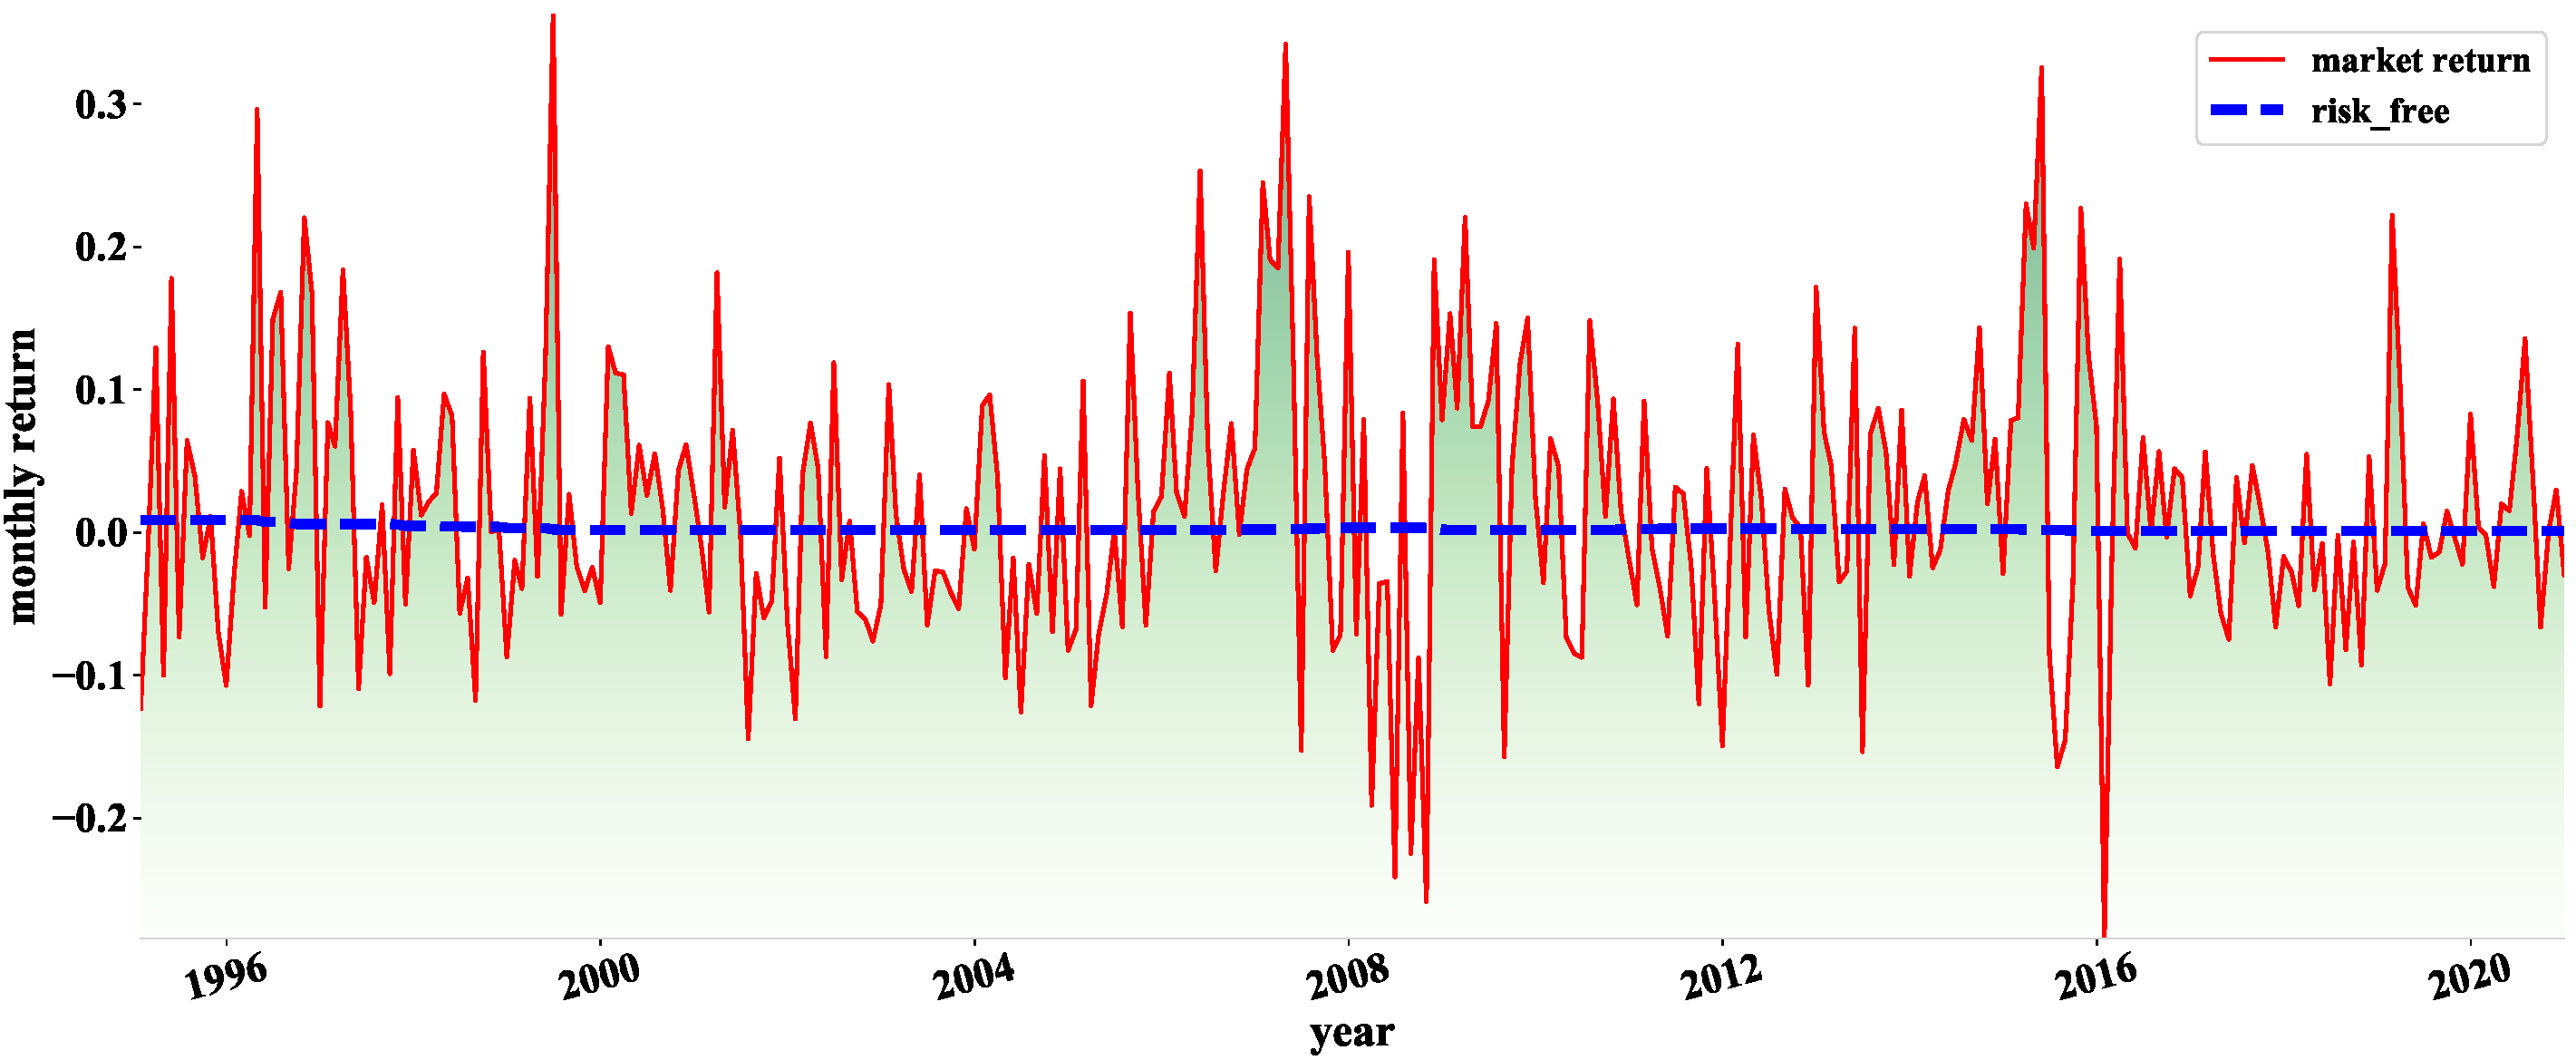
\includegraphics[scale=0.31]{market_return.pdf}
		\caption{市场组合月收益率表现}
		\label{marketret}
	\end{figure}

	图\ref{marketret}为市场组合的月收益率表现,反应的是从1996到2020年的整个股票市场大盘的收益率变化情况,从图中可以看出股票市场的波动十分大,有时月度的收益率能够在30\%以上,有时甚至低于-20\%,比如在2008年金融危机的时候。从表\ref{biao2}的描述统计来看,股票市场组合的平均年化收益率约为14\%,单月收益率约为1.17\%,月波动率即标准差为9.6\%,对应的夏普比率为0.179,可以看出市场组合的收益率相对于无风险利率而言较为可观,但存在波动性过大的问题,导致夏普比率不高。
	
	\begin{table}[ht]
		\centering
		\caption{市场组合收益率的描述统计}
		\begin{tabular}{ccccc}
			\hline
			& 平均年化收益率 & 平均月化收益率 & 月波动率  & 夏普比率  \\ \hline
			市场组合 & 14\%    & 1.17\%  & 9.6\% & 0.179 \\ \hline
		\end{tabular}
		\label{biao2}
	\end{table}
	
	图\ref{marketret}中的蓝色虚线表示的是单月无风险收益率,无风险收益率指的是没有风险的收益率,不存在违约的情况,一般使用国库券利率来表示,可以看出无风险利率相较于市场收益率曲线波动不大,自2015年12月至今单月无风险利率约为0.124\%,相对于股票市场组合单月平均收益率1.17\%,收益是比较小的,但是特点是十分稳定。
	
	\subsection{投资组合构造}
	我们首先利用线性回归和XGboost等机器学习,股票特征为输入特征,对股票价格进行预测。机器学习方法都需要对模型中的参数进行训练,比如线性回归中参数。这里我们采用12个月周期的滚动期来对模型的参数进行训练。举例而言,当我们在预测2018年1月股价收益率的时候,我们的输入特征是2017年12月份股票的特征,这时我们需要对参数进行训练,我们利用的是2017年1至12月的股价收益率,以及2016年12月与2017年1至11月的股票特征来对模型进行训练,通过以往这12个月的数据来拟合出模型的参数,进而用于预测。
	
	在得到预测的股票收益率之后,我们做多收益率最高前10\%的股票,做空收益率最低前10\%的股票,这样可以得到一个投资组合。即我们购买持有收益率最高10\%的股票,然后借入收益率最低10\%的股票卖出,然后再还股票,形成一个投资组合。总而言之,做多的股票,我们得到的收益率就是做多股票的收益率$r_l$,股票涨多少,我们就赚多少;而做空的股票,我们得到的收益率就是多空股票的收益率$r_s$的负数,股票跌多少,我们赚多少。
	\begin{equation}
		r_{ls}=r_l-r_s \label{E4.3}
	\end{equation}
	因此整个投资组合的收益率$r_{ls}$即可以由\eqref{E4.3}所表示,对应的含义是我们构造的多空投资组合,其收益率$r_{ls}$,一部分来自于做多股票的收益率$r_l$,多头股票一般是我们指做多的股票,多头涨多少,我们赚多少;另一部分来自于做空股票的收益率$-r_s$,空头股票一般是我们做空的股票,空头跌多少,我们赚多少。
	
	线性回归和XGboost具体实现可以调用Python中的sklearn.linear\_model包中的 LinearRegression和xgboost.sklearn包中XGBRegressor进行实现。
	
	从表\ref{biao3}和表\ref{biao4},我们可以得到线性回归和XGboost构造的投资组合的表现。线性回归构造的投资组合,多空头寸投资组合平均年化收益率为31.5\%,并且由t值7.75可知收益率显著大于0,FF3收益率是指风险调整后的收益率大小,对应的FF3收益率为28\%,相应的夏普比率为1.78。XGboost算法构造的投资组合,多空头寸投资组合平均年化收益率为38.8\%,并且由t值9.76可知收益率显著大于0,FF3收益率是指风险调整后的收益率大小,对应的FF3收益率为35.1\%,相应的夏普比率为2.2. 
	\begin{table}[ht]
		\small
		\caption{线性回归构造的投资组合表现}
		\label{biao3}
		\begin{tabular}{cccccc}
			\hline
			& 年化收益率   & 收益率t-value & FF3收益率 & FF3收益率t-value & 夏普比率  \\ \hline
			Long\_Short & 31.5\%  & 7.75       & 28\%   & 7.46          & 1.78  \\
			Long        & 31.2\%  & 3.69       & 14\%   & 5             & 0.81  \\
			Short       & -0.19\% & -0.03      & -1.6\% & -6.6          & -0.08 \\ \hline
		\end{tabular}
	\end{table}
	
	\begin{table}[ht]
		\small
		\caption{XGboost构造的投资组合表现}
		\label{biao4}
		\begin{tabular}{cccccc}
			\hline
			& 年化收益率  & 收益率t-value & FF3收益率 & FF3收益率t-value & 夏普比率  \\ \hline
			Long\_Short & 38.8\% & 9.76       & 35.1\% & 9.44          & 2.2   \\
			Long        & 36.7\% & 4.18       & 19\%   & 6.58          & 0.94  \\
			Short       & -2\%   & -0.27      & -18\%  & -8.32         & -0.13 \\ \hline
		\end{tabular}
	\end{table}
	
		\begin{figure}[ht]
		
		\centering
		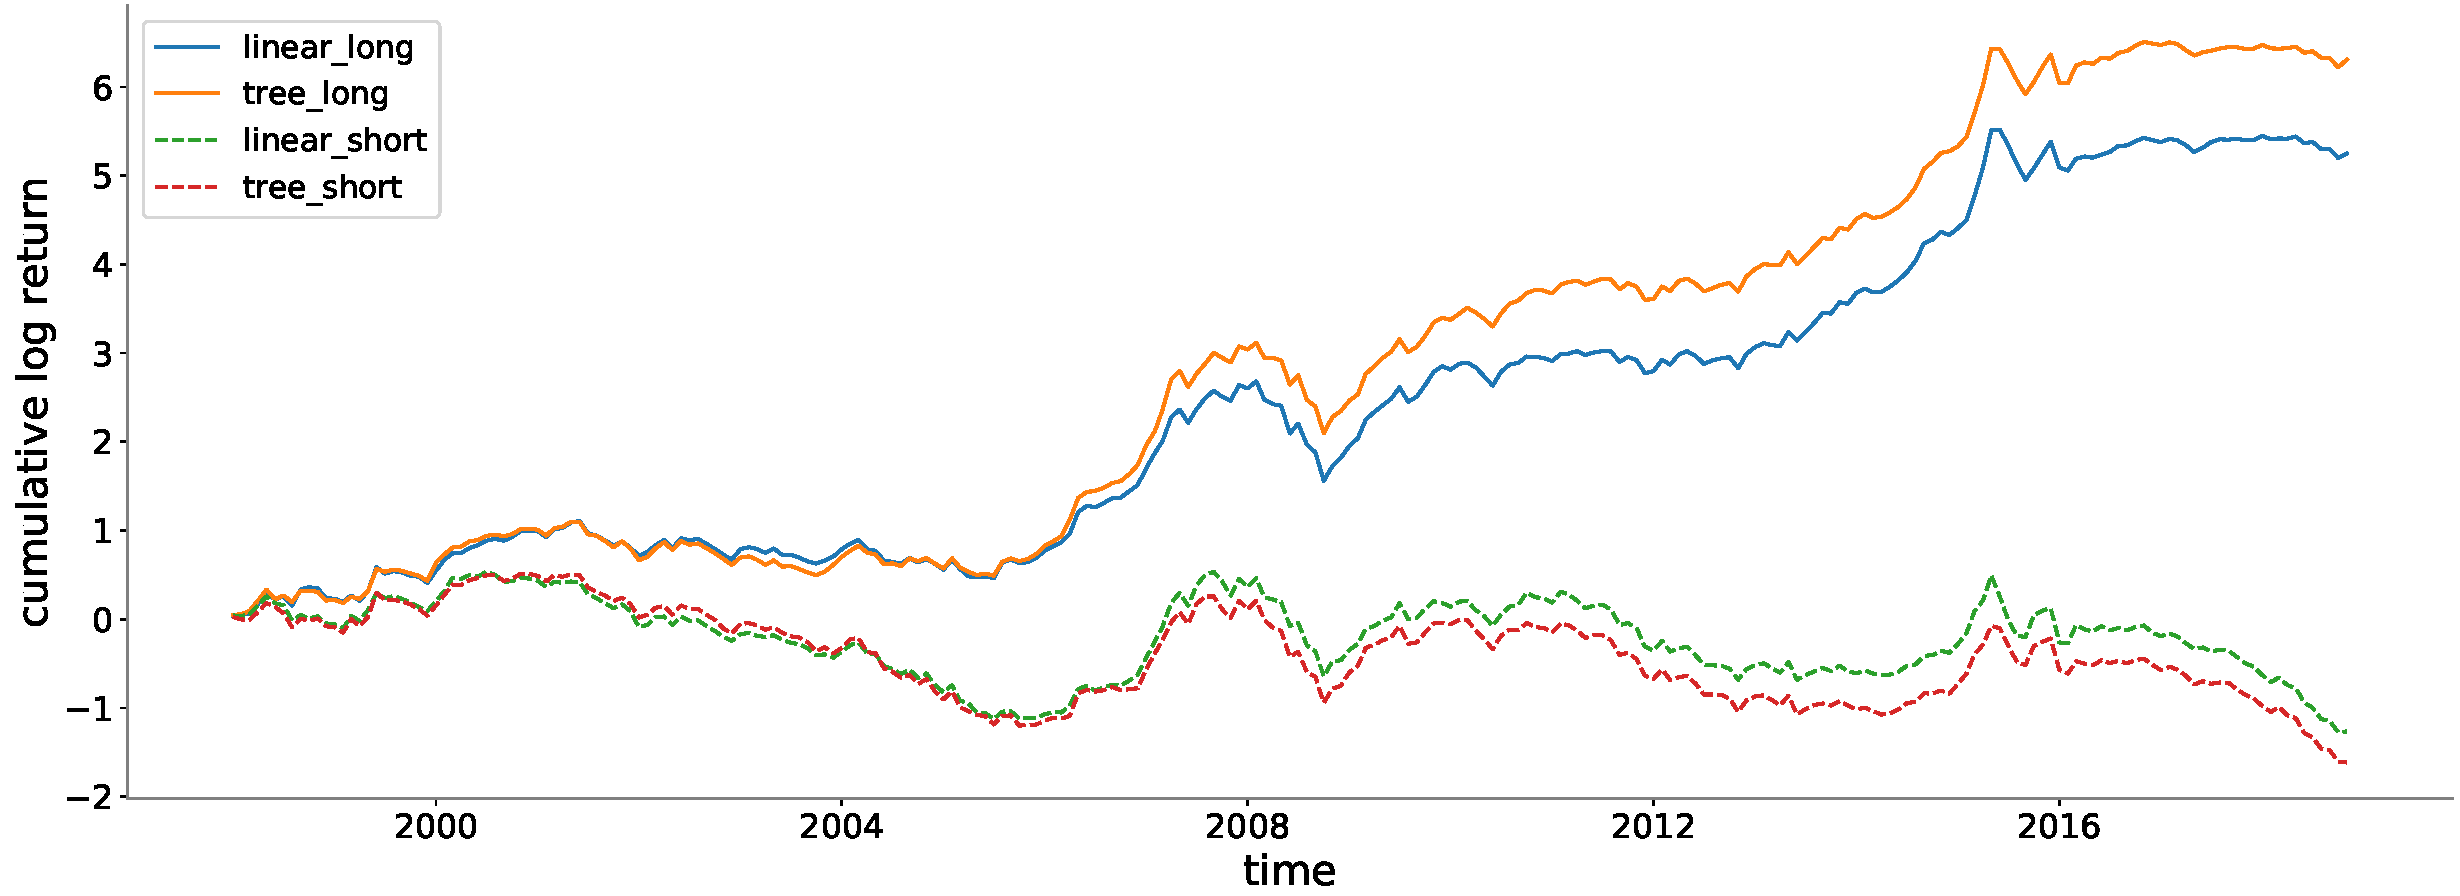
\includegraphics[scale=0.36]{linear_tree_long_short.pdf}
		\caption{线性回归和XGboost投资组合的多头和空头累计对数收益率}
		\label{linear_tree_long_short}
	\end{figure}
	
	\begin{figure}[ht]
		
		\centering
		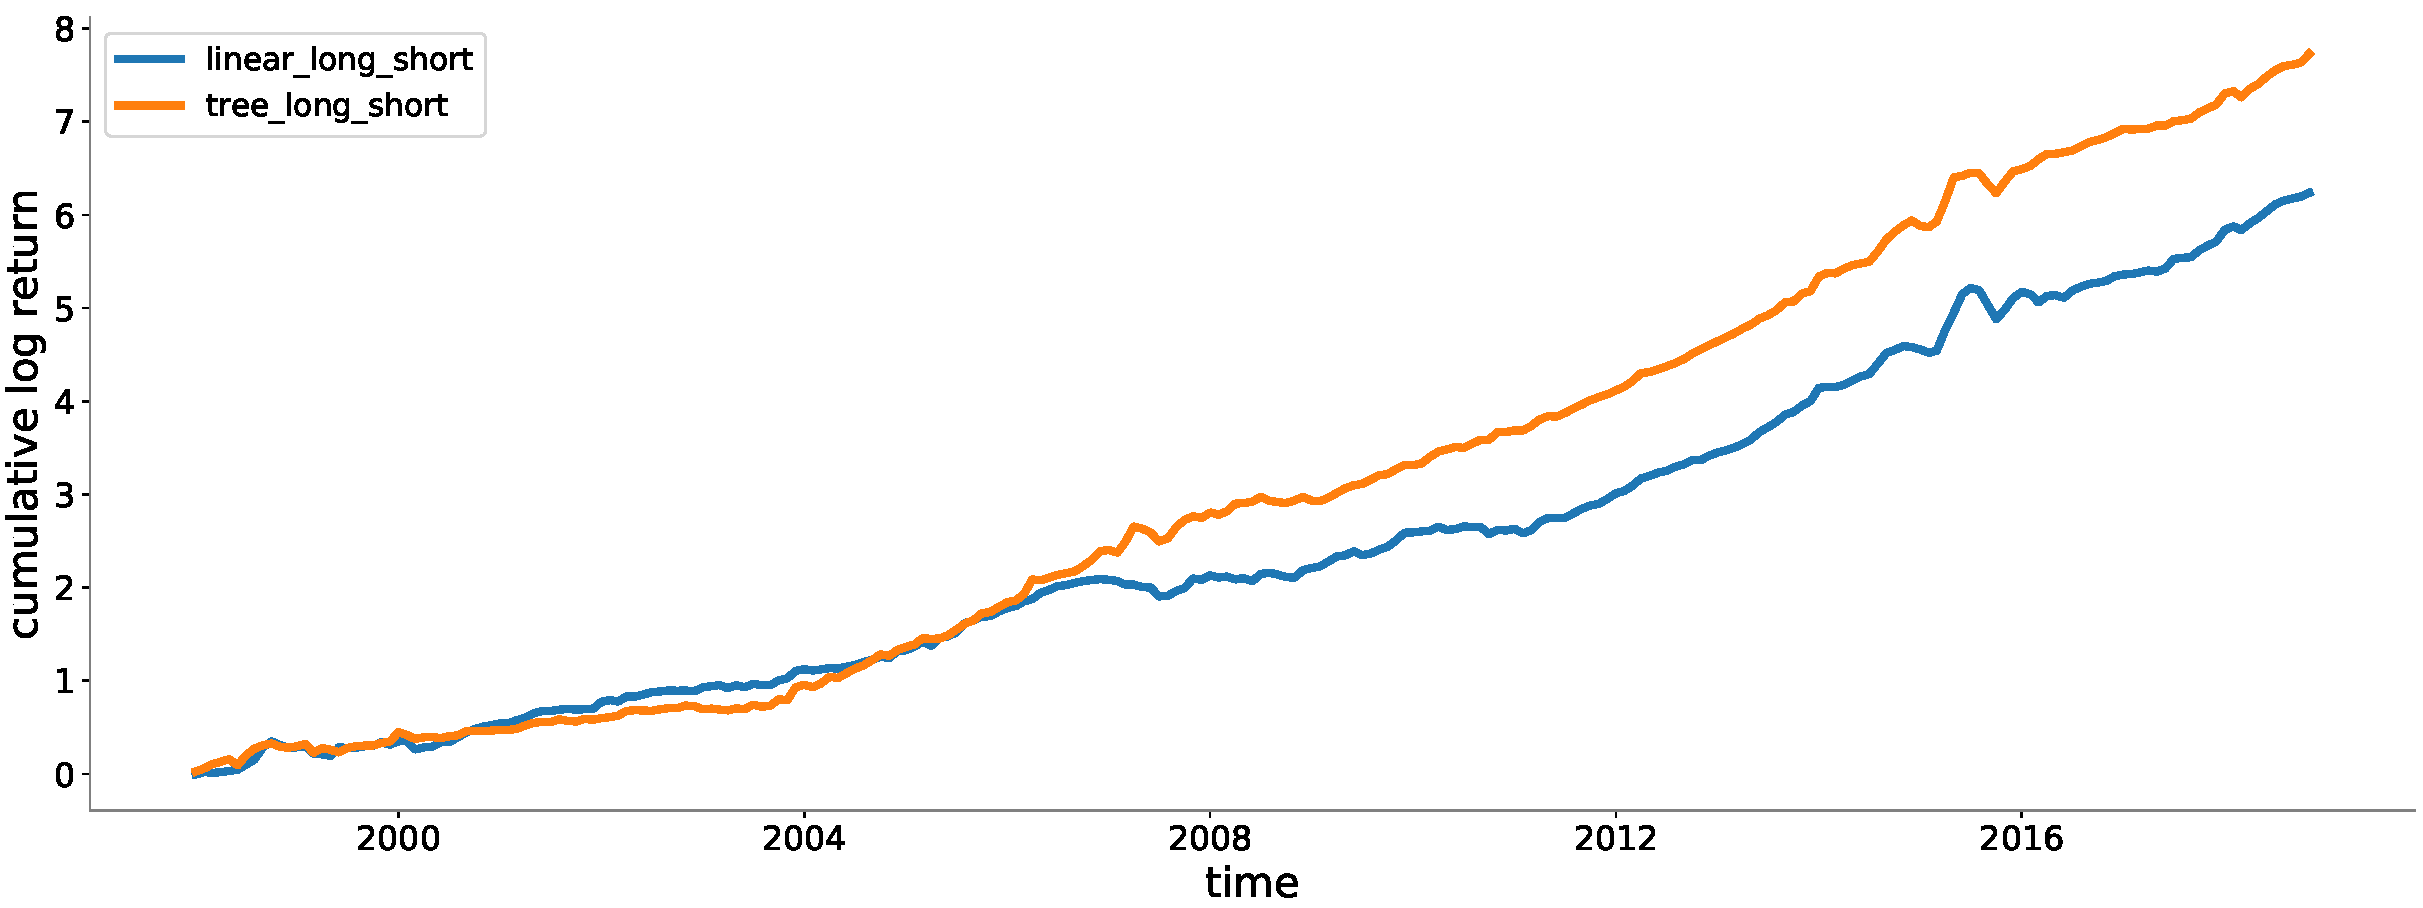
\includegraphics[scale=0.37]{Linear_tree_ls.pdf}
		\caption{线性回归和XGboost投资组合的多空头累计对数收益率}
		\label{linear_tree_ls}
	\end{figure}
	
	其中表\ref{biao3}和表\ref{biao4}中Long是指多头,Short是指空头,Long\_Short则代表是多空头寸。相较于\ref{S4.2}节的市场基准组合,线性回归构造的投资组合收益率约为市场组合收益率的2.25倍,夏普比率约为9倍;XGboost构造的投资组合收益率约为市场组合的2.77倍,夏普比率为11倍左右。两种算法得到的投资组合无论在收益率,还是稳定性上,都得到了很大的提升。
	
	\begin{equation}
		log\_ret = log(1+r) \label{E4.19}
	\end{equation}
	
	从图\ref{linear_tree_long_short}中,我们可以看出通过线性回归和XGboost构造的投资组合中多头和空头的累计对数收益率,即做多股票(多头)和做空股票(空头)的收益率。对数收益率即可以由\eqref{E4.19}表示,即收益率$r$加1后取对数,累计对数收益率则指的是加多个时期的对数收益率相加得到的值。从图\ref{linear_tree_long_short}可以知道,从1998到2018年这20年的时间中,线性回归得到多头头寸升值为原来的exp(5.247)=190倍,XGboost投资组合升值为原来的exp(6.308)=548.9倍。而图\ref{linear_tree_ls}反应的则是多空组合的累计对数收益率,其中多空组合的收益率由式子\eqref{E4.3}所定义,即$r_{ls}=r_l-r_s$,可以看出多空组合收益率更高,且一路上升较为稳定。
	
	
	%下面我们再对神经网络方法构造的投资组合进行分析,神经网络的训练可以利用Python中Pytorch来进行实现。我们分别比较4层神经网络算法得到的性能效果,当神经网络为1层时,神经元个数为64;神经网络为2层时,神经元个数为64,32;神经网络为3层时,神经元个数为64,32,16;神经网络为4层,神经元个数为64,32,16,8,即神经元个数随着网络层面按幂次递减。
	
	
	\subsection{变量选择后投资组合分析 \label{S4.4}}
	在\ref{S4.4}节中,我们分析变量数目对投资组合的收益率,夏普比率等表现的影响,并且比较变量数目对程序运行时间的影响,其中在选择变量作为输入特征时,我们将利用\ref{S3.2}节中贝叶斯选择变量得到的结论。
	
	程序运行环境如下:电脑型号为MacBook Air (13-inch, 2017),处理器为1.8 GHz Intel Core i5,内存为8 GB 1600 MHz DDR3,
	
	
	\begin{figure}[ht]
		
		\centering
		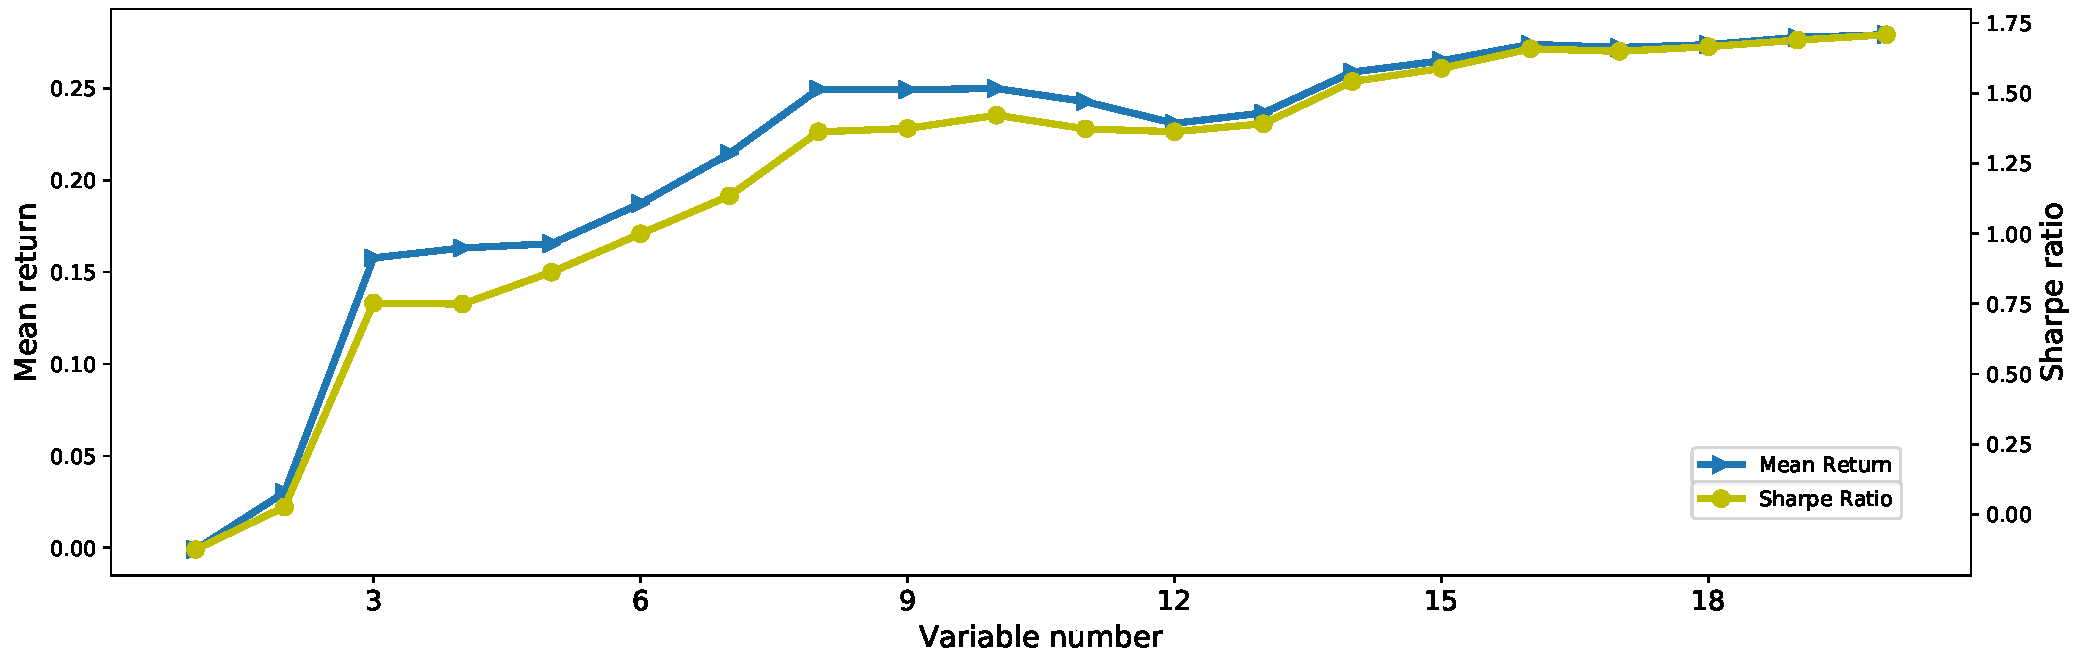
\includegraphics[scale=0.45]{linear_ret_var.pdf}
		\caption{线性回归投资组合中变量数目与年化收益率、夏普比率的关系}
		\label{linear_var_ret}
	\end{figure}
	
	\begin{figure}[ht]
		
		\centering
		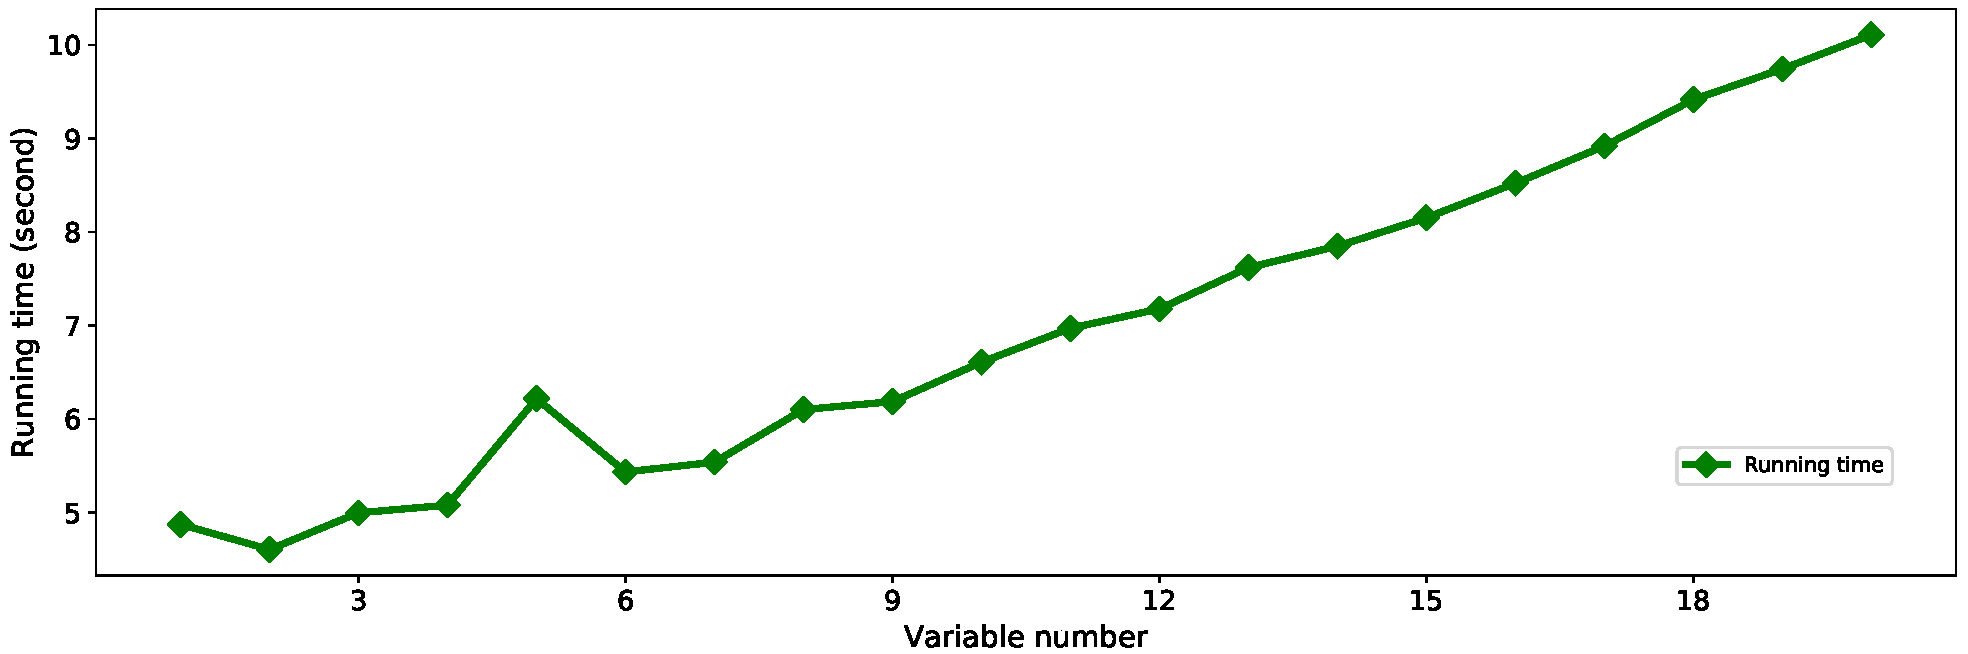
\includegraphics[scale=0.455]{linear_running.pdf}
		\caption{线性回归投资组合中变量数目与程序运行时间的关系}
		\label{linear_running}
	\end{figure}
	
	我们将\ref{S3.2}节中贝叶斯方法选取的变量作为输入特征即自变量,依次将对应的变量纳入预测模型当中,对收益率进行预测。然后,我们做多收益率最高10\%的股票,做空收益率最低10\%的股票,构造一个多空头寸的投资组合,并且对投资组合的收益率、夏普比率和对应程序运行时间进行分析。
	
	从图\ref{linear_var_ret}可以看出,由线性回归算法构造的投资组合平均年化收益率和夏普比率随着变量数目的上升而上升,在13个变量之后趋于平稳。投资组合的年化收益率和夏普比率在变量为1-9个时候,随着变量数目增加上升较快,在用前9个变量作为自变量进行线性回归而构造投资组合时,对应投资组合的年化收益率为25\%,夏普比率为1.37,当使用前20个变量来构造投资组合时,对应的年化收益率为28\%,夏普比率为1.7,已经与使用全部自变量(35个)来构造投资组合的效果类似。另一方面,我们可以从图\ref{linear_running}看出,线性回归中程序的运行时间随着变量数目增加而增加,增长速度大致成线性关系,程序运行20个自变量所需要的时间大概为10s,可以看出线性回归的程序运行时间相对较小。
	
	\begin{figure}[ht]
		
		\centering
		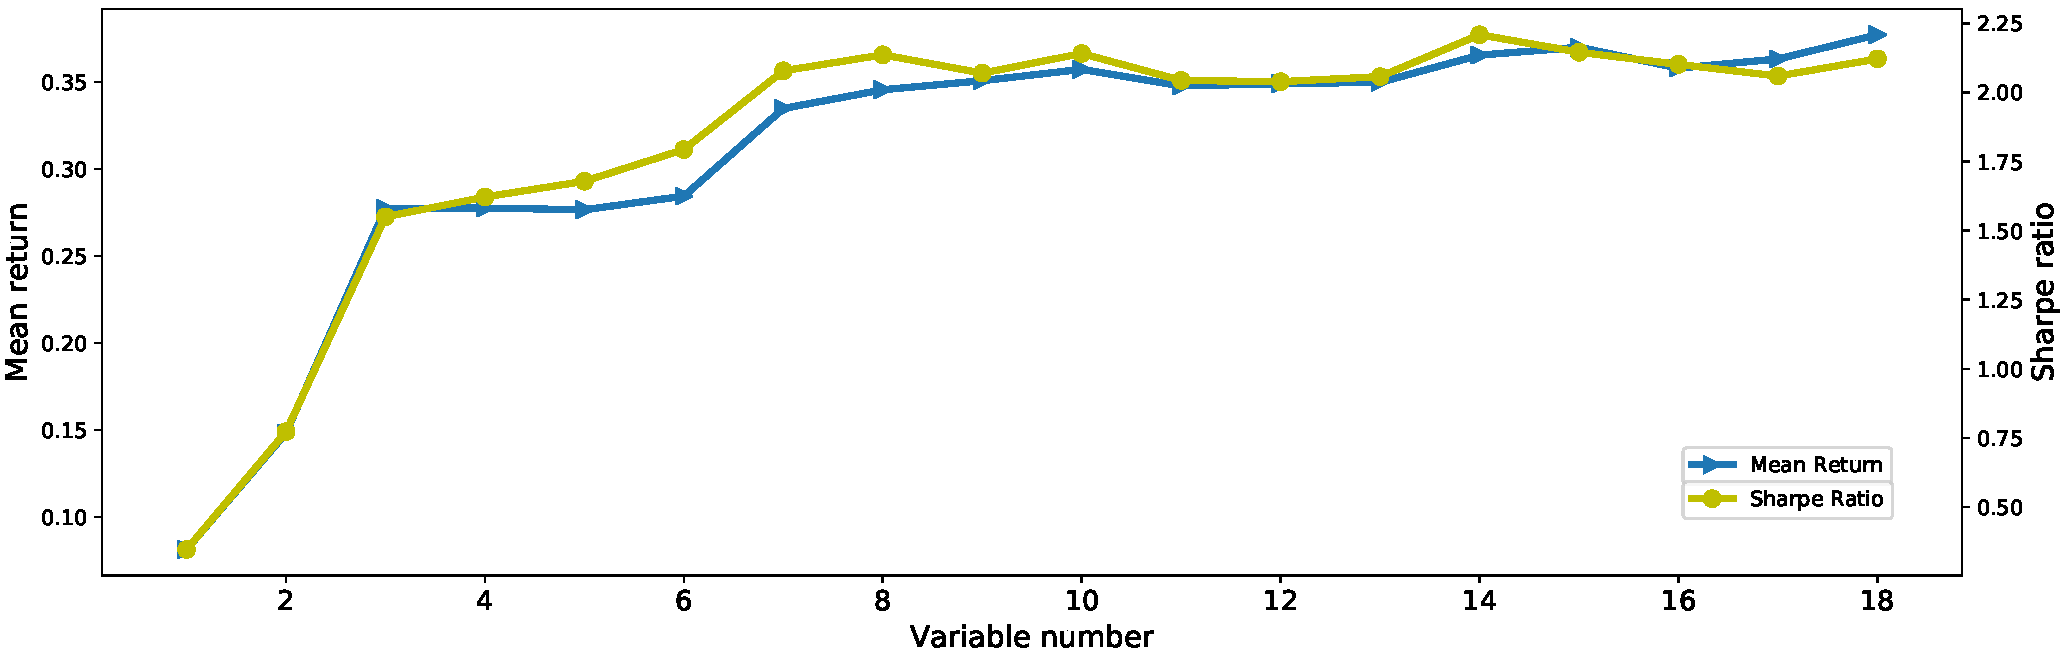
\includegraphics[scale=0.45]{xgboost_var_ret.pdf}
		\caption{XGboost投资组合中变量数目与年化收益率、夏普比率的关系}
		\label{xgboost_var_ret}
	\end{figure}
	
	\begin{figure}[ht]
		
		\centering
		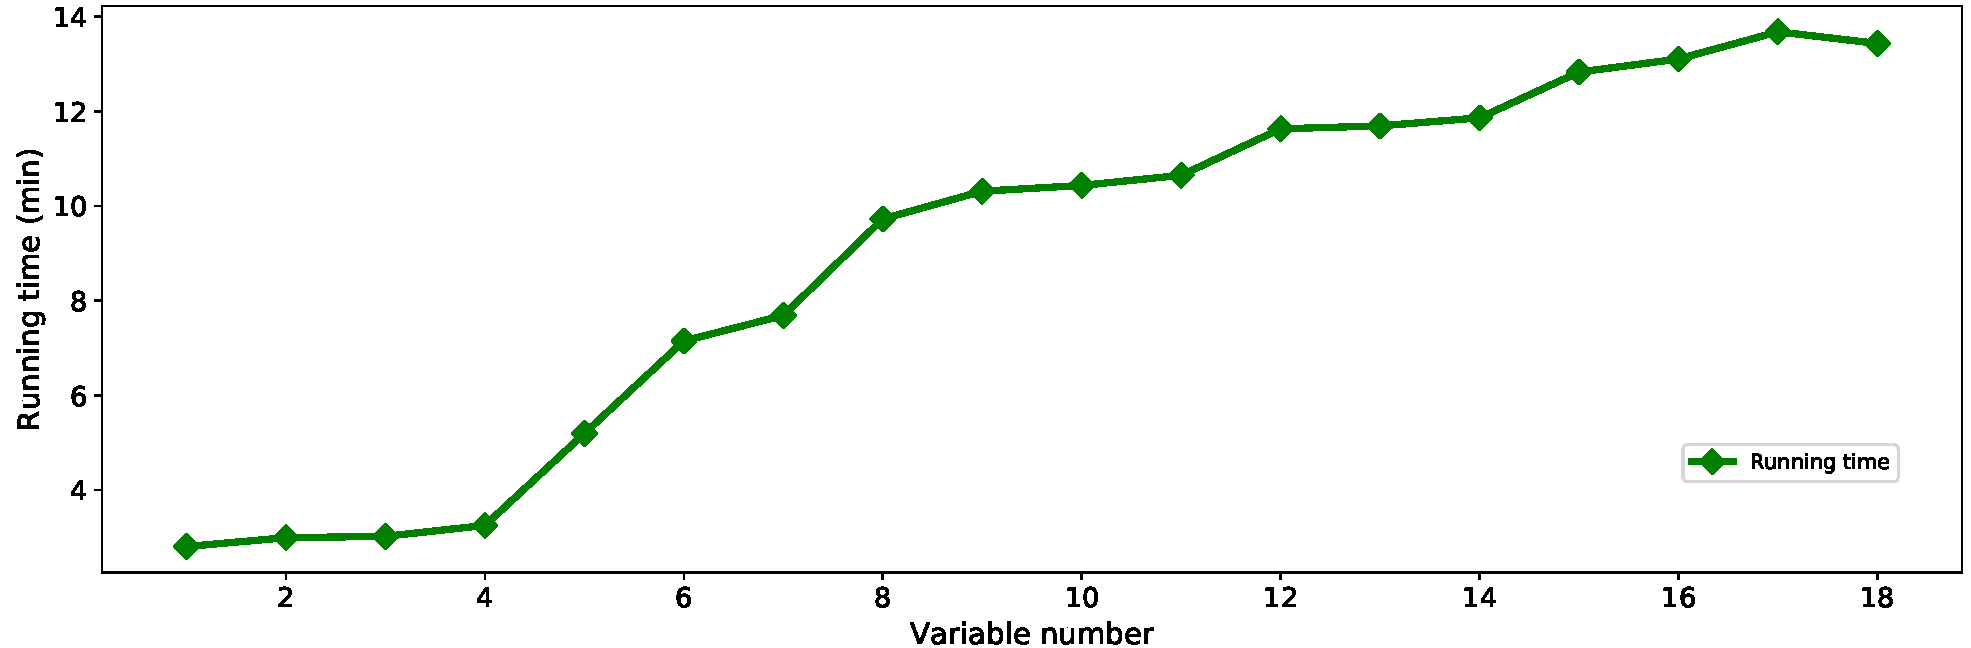
\includegraphics[scale=0.45]{xgboost_running.pdf}
		\caption{XGboost投资组合中变量数目与程序运行时间关系}
		\label{xgboost_running}
	\end{figure}
	
	从图\ref{xgboost_var_ret}中,可以发现利用XGboost算法构造投资组合中,随着利用的变量个数增加,平均年化收益率和夏普比率都有一定的提升,而后趋于稳定。在1-7个变量之间,年化收益率随着使用变量数目增长速度较快,我们使用前面7个变量对收益率进行预测,做多收益率最高10\%的股票,做空收益率最低10\%的股票,对应投资组合的年化收益率为33\%,对应夏普比率为2.07。而变量数目在7个以后时,投资组合收益率和夏普比率随着变量数目增加,上升不再明显,说明后面变量预测的边际效能在慢慢降低。当使用18个变量进行构造投资组合时,对应的年化收益率为0.377\%,夏普比率为2.12,已经与使用全部变量(共35个)个变量的效果十分类似。从图\ref{xgboost_running}中,我们也可以发现时间运行时间随着变量个数增加而增加,而且需要的时间较长,当利用18个变量来构造投资组合时,程序已经需要运行13.4分钟了。
	
	从上述实验中,我们可以发现通过变量选择方法可以提高模型训练的速度,减少训练所用的时间,而且只需要用16个变量,相当于所有变量总和的一半,来进行训练模型,即可以得到和全部变量(35个)相近的年化收益率和夏普比率。XGboost树模型在训练上使用的时间大概是线性回归的60倍,但其构造的投资组合,在年化收益率和夏普比率等方面均优于线性回归方法,能够较好捕抓非线性结构。
	
	\newpage
	\section{总结与展望}
	本文对中国A股市场进行分析,对1998-2018年的股票收益率和公司特征等数据进行处理,通过贝叶斯变量选择方法寻找出中国A股市场中重要的定价因子,并利用机器学习方法对收益率进行预测,以此来构造投资组合。
	
	在第\ref{S3}节中,我们利用贝叶斯变量选择方法对定价因子进行选择,并发现对股价具有驱动作用的重要因子。我们首先介绍贝叶斯变量选择的思想与原理,在线性回归中通过贝叶斯方法选取重要变量由Mitchell和Beauchamp(1988)较早地提出,其假设回归系数$\boldsymbol{\beta}$服从spike and slab的先验分布,并计算出模型$A_m$的后验分布,选择出最大的后验概率的模型。我们运行R中spikeslab包发现在所有定价因子即变量当中,收益率波动率、最大日收益率、交易额波动率、账面市值比、总资产周转率和总波动率等变量对股价收益率具有较好的预测效力,并且通过贝叶斯方法选择出的变量和LASSO方法选择出的变量相近似。
	
	在第\ref{S4}节中,我们通过机器学习方法对股价收益率进行预测,并构造投资组合。我们选取了两种典型的预测方法,一种是线性回归模型,另一种是能够较好地捕抓数据非线性结构的XGboost树模型。我们首先通过预测方法对股价收益率进行预测,做多预测收益率最高10\%的股票,做空收益率最低的10\%的股票,形成一个多空头的投资组合。利用线性回归模型构造的投资组合,年化收益率约为31.5\%,夏普比率为1.78,而利用XGboost算法构造的投资组合,年化收益率约为38.8\%,夏普比率为2.2,XGboost算法能得到表现更好的投资组合,但是训练时间较线性回归较长,而通过变量选择方法得到的变量,只需要用到一半的变量即可得到较好的效果,并减少模型训练的时间。
	
	总结而言,本文通过实证分析发现了中国A股市场中重要的定价因子,并探究了机器学习用于构造投资组合的性能表现。在未来研究中,还可以进行如下的探索,在本文中只利用到了35个中国A股市场的定价因子,可以考虑构造更多的定价因子来继续探索,另外,本文选取线性回归和XGboost两种典型的预测算法来探究,未来可以尝试比较其他更多的算法,比如神经网络和深度学习等各种机器学习算法在构造投资组合中的表现。
	
	\newpage
	\section{致谢}
	四年的时间转眼而过,虽然作为一个商科的学生,但一直怀揣着对理工学科的热爱。在最初刚上大一的时候,贾宝国老师的高数课和胡国权老师的线代课点燃了我大学时期对数学的热情,自己也因为热爱数学当上了线代课的课代表,有幸在大二时候能够辅修统计,大三时候双学位数学与应用数学,直到现在能够顺利毕业,一路上满怀感恩。
	
	双学位数学的日子虽然比较辛苦,但在这段时光对我来说却是一个美好的回忆。学习两个专业的知识意味着要牺牲一些休息娱乐的时间,完成本专业任务之后,周末也要开始温习在数院学习过的知识,到了考试周也要考双倍的考试。但是这个过程中我是十分开心的,学习的过程中遇到茼神、国哥和怡姐等等的好朋友,大家也十分耐心,经常帮我解决不懂的知识。也还记得在数院认识了大学中最好的朋友润泽,大二时一起打数模比赛,大三时候在宋雷老师教授的运筹学课上一起组队写小组大作业,清晰地记得展示前的一天晚上疯狂改稿,排练ppt到2点的样子,最后也是因为默契与努力,在运筹学拿到了最高分。是的,转眼临近毕业了,茼神和国哥去了香港和新加坡读数学PhD,润泽也如愿以偿去了清华,不知道什么时候才能再看见数院的这些好朋友了,怀念和国哥一起打球,还有和润泽聊天的时光,祝愿大家都能够未来顺利。
	
	同时也感谢数院老师们一路上的指导与帮助,让我在数学学习上取得了很大的进步。嘉哥讲的数学实验与数学软件,蔡敬衡老师将的多元统计分析与应用等等都留给了我很深刻的印象,也将我的数学基础一步步提高。同时也十分感谢指导我毕业论文的刘老师,无论是从刘老师教授的数学分析课程,还是从论文指导的过程中,都可以体会感受到老师是个幽默善良,对生活充满热爱的人。四年数学学习也让我的数理基础得到了很大的改进,对未来研究生的学习大有帮助。
	
	我会永远记住这段美好的时光,在我最青春的大学四年中,和好朋友一起学习数学知识,一起做题,并且有幸遇到这么多好的老师和同学们,这些每个积极向上,热情洋溢的日子都是如此的美好。
	
	\newpage
	%\bibliographystyle{unsrtnat}
	\bibliographystyle{unsrtnat}
	\bibliography{math2}
	
	\newpage
	\section{附录}
	
	\subsection{数学公式证明}
	\noindent
	\textbf{公式推导1:}
	
	\textbf{这里,我们给出从\eqref{E3.9}到\eqref{E2.9}的推导过程},首先\eqref{E3.9}如下式所示,
	
	\begin{equation*}
		\begin{aligned}
			&p\left(\mathbf{y} \mid A_{m}, \boldsymbol{\beta}_{m}, \sigma\right)=(2 \pi)^{-n / 2} \sigma^{-n} \\
			&\quad \times \exp \left[-\frac{1}{2 \sigma^{2}}\left(S_{m}^{2}+\left(\boldsymbol{\beta}_{m}-\hat{\boldsymbol{\beta}}_{m}\right)^{\prime} \mathbf{X}_{m}^{\prime} \mathbf{X}_{m}\left(\boldsymbol{\beta}_{m}-\hat{\boldsymbol{\beta}}_{m}\right)\right)\right] 
		\end{aligned}
	\end{equation*}
	我们将\eqref{E3.9}乘以$p(\boldsymbol{\beta}_m \mid A_m,\sigma)=\prod_{J_{m}}\left(2 f_{j}\right)^{-1} $,可以得到
	\begin{equation*}
		\begin{aligned}
			&p\left(\mathbf{y}, \boldsymbol{\beta}_{m} \mid A_{m}, \sigma\right)=\prod_{J_{m}} \left(2 f_{j}\right)^{-1}  (2 \pi)^{-n / 2} \sigma^{-n} \\
			&\quad \times \exp \left[-\frac{1}{2 \sigma^{2}}\left(S_{m}^{2}+\left(\boldsymbol{\beta}_{m}-\hat{\boldsymbol{\beta}}_{m}\right)^{\prime} \mathbf{X}_{m}^{\prime} \mathbf{X}_{m}\left(\boldsymbol{\beta}_{m}-\hat{\boldsymbol{\beta}}_{m}\right)\right)\right] 
		\end{aligned}
	\end{equation*}
	我们在上式中对$\boldsymbol{\beta}_m$进行积分,注意$\boldsymbol{\beta}_m$是一个$k_m$维向量,所以这个积分是$k_m$维积分,由于每个$\beta_{j}$的范围都是$(-\infty,\infty)$,故多重积分区域为$R^{k_m}$
	\begin{equation*}
		p\left(\mathbf{y} \mid A_{m}, \sigma\right)= \int_{R^{k_m}} p\left(\mathbf{y}, \boldsymbol{\beta}_{m} \mid A_{m}, \sigma\right) d \boldsymbol{\beta}_{m}
	\end{equation*}
	下面求解该积分
	\begin{equation*}
		\begin{aligned}
			&p\left(\mathbf{y} \mid A_{m}, \sigma\right)=\int_{R^{k_m}}  \prod_{J_{m}} \left(2 f_{j}\right)^{-1}  (2 \pi)^{-n / 2} \sigma^{-n} \\
			&\quad \times \exp \left[-\frac{1}{2 \sigma^{2}}\left(S_{m}^{2}+\left(\boldsymbol{\beta}_{m}-\hat{\boldsymbol{\beta}}_{m}\right)^{\prime} \mathbf{X}_{m}^{\prime} \mathbf{X}_{m}\left(\boldsymbol{\beta}_{m}-\hat{\boldsymbol{\beta}}_{m}\right)\right)\right] d \boldsymbol{\beta}_m
		\end{aligned}
	\end{equation*}
	其中$\hat{\boldsymbol{\beta}}_{m}$在积分中相当于常数,可以做变量替换$\mathbf{c}_m = \boldsymbol{\beta}_m -\hat{\boldsymbol{\beta}}_m$,因此积分可以转换为
	\begin{equation*}
		\begin{aligned}
			&p\left(\mathbf{y} \mid A_{m}, \sigma\right)=\int_{R^{k_m}}  \prod_{J_{m}} \left(2 f_{j}\right)^{-1}  (2 \pi)^{-n / 2} \sigma^{-n} \\
			&\quad \times \exp (-\dfrac{1}{2\sigma^2} S_m^2) \times \exp \left[ -\dfrac{1}{2\sigma^2  } \mathbf{c}_m^{\prime}  \mathbf{X}_{m}^{\prime} \mathbf{X}_{m} \mathbf{c}_m \right] d \mathbf{c}_m
		\end{aligned}
	\end{equation*}
	我们将常数提到积分号外面,可以得到
	\begin{equation*}
		\begin{aligned}
			&p\left(\mathbf{y} \mid A_{m}, \sigma\right)=  \prod_{J_{m}} \left(2 f_{j}\right)^{-1}  (2 \pi)^{-n / 2} \sigma^{-n} \\
			&\quad \times \exp (-\dfrac{1}{2\sigma^2} S_m^2) \int_{R^{k_m}} \exp \left[ -\dfrac{1}{2\sigma^2  } \mathbf{c}_m^{\prime}  \mathbf{X}_{m}^{\prime} \mathbf{X}_{m} \mathbf{c}_m \right] d \mathbf{c}_m
		\end{aligned}
	\end{equation*}
	注意到$ \mathbf{X}_{m}^{\prime} \mathbf{X}_{m}$是可以进行分解的,我们将$ \mathbf{X}_{m}^{\prime} \mathbf{X}_{m}$分解为$\mathbf{U}^{\prime} \mathbf{D} \mathbf{U}$,其中$\mathbf{D}$是对角矩阵,并且我们再做一次变量替换,令$\mathbf{w} = \mathbf{U} \mathbf{c}_m$,相当于$\mathbf{w}$是$\mathbf{c}_m$的一个线性变换,然后可以得到
	$$\mathbf{c}_m^{\prime}  \mathbf{X}_{m}^{\prime} \mathbf{X}_{m} \mathbf{c}_m = \mathbf{c}_m^\prime \mathbf{U}^{\prime} \mathbf{D} \mathbf{U} \mathbf{c}_m = \mathbf{w}^\prime \mathbf{D} \mathbf{w}$$
	注意到$\mathbf{D}$是对角矩阵,因此有$\mathbf{w}^\prime \mathbf{D} \mathbf{w} = \Sigma_{i=1}^{k_m} \sigma_i w_i^2$,可以得到
	\begin{equation*}
		\begin{aligned}
			\int_{R^{k_m}} \exp \left[ -\dfrac{1}{2\sigma^2  } \mathbf{c}_m^{\prime}  \mathbf{X}_{m}^{\prime} \mathbf{X}_{m} \mathbf{c}_m \right] d \mathbf{c}_m = \int_{R^{k_m}} \exp ( -\dfrac{1}{2\sigma^2  } \mathbf{w}^\prime \mathbf{D} \mathbf{w} ) \mid J \mid d \mathbf{w}_m
		\end{aligned}
	\end{equation*}
	其中雅可比行列式$\mid J \mid = \mid \mathbf{U} \mid$,由正交分解可以知道行列式$\mid \mathbf{U} \mid$只能为1或-1,而此处对应的值为1,因此$\mid J \mid = 1$,因此积分求解转换下式
	\begin{equation*}
		\begin{aligned}
			\int_{R^{k_m}} \exp ( -\dfrac{1}{2\sigma^2  } \mathbf{w}^\prime \mathbf{D} \mathbf{w} ) \mid J \mid d \mathbf{w}_m &= \int_{R^{k_m}} \exp ( -\dfrac{1}{2\sigma^2  } \Sigma_{i=1}^m \sigma_i w_i^2) d \mathbf{w}_m \\
			&= \prod_{i=1}^{k_m} \int_{R^1} \exp ( -\dfrac{1}{2\sigma^2  } \sigma_i w_i^2) d w_i \\
		\end{aligned}
	\end{equation*}
	再做一次变量替换$t_i = \dfrac{\sqrt{\sigma_i } w_i }{\sqrt{2} \sigma}$,可以得到
	\begin{equation*}
		\begin{aligned}
			\prod_{i=1}^{k_m} \int_{R^1} \exp ( -\dfrac{1}{2\sigma^2  } \sigma_i w_i^2) d w_i &= \prod_{i=1}^{k_m} \left( \dfrac{\sqrt{2} \sigma}{\sqrt{\sigma_i}}  \int_{R^1} \exp(-t_i^2) dt_i  \right)
		\end{aligned}
	\end{equation*}
	其中由$\prod_{i=1}^{k_m} \sqrt{\sigma_i} = \sqrt{det(\mathbf{D})} = \sqrt{\mid \mathbf{X}^\prime \mathbf{X}\mid}$,并且由$\int_{R^1} \exp(-t_i^2) dt_i =\sqrt{\pi} $可以知道
	\begin{equation*}
		 \prod_{i=1}^{k_m} \left( \dfrac{\sqrt{2} \sigma}{\sqrt{\sigma_i}}  \int_{R^1} \exp(-t_i^2) dt_i  \right) = \dfrac{2^{k_m/2} \sigma^{k_m}}{\mid \mathbf{X}^\prime \mathbf{X} \mid^{1/2} } \pi^{k_m/2}
	\end{equation*}
	综上,可以得到\eqref{E2.9}式子
	\begin{equation*}
		\begin{aligned}
			&p\left(\mathbf{y} \mid A_{m}, \sigma\right)=\left(\prod_{J_{m}}\left(2 f_{j}\right)^{-1}\right) \\
			&\times(2 \pi)^{-\left(n-k_{m}\right) / 2}\left|\mathbf{X}_{m}^{\prime} \mathbf{X}_{m}\right|^{-1 / 2} \sigma^{-\left(n-k_{m}\right)} \exp \left[-S_{m}^{2} /\left(2 \sigma^{2}\right)\right] 
		\end{aligned}
	\end{equation*}
	~\\ \\
	\textbf{公式推导2:}
	
	在公式推导2中,\textbf{我们给出从\eqref{E2.9}到\eqref{E2.10}的推导过程},首先\eqref{E2.9}如下式所示
	\begin{equation*}
		\begin{aligned}
			&p\left(\mathbf{y} \mid A_{m}, \sigma\right)=\left(\prod_{J_{m}}\left(2 f_{j}\right)^{-1}\right) \\
			&\times(2 \pi)^{-\left(n-k_{m}\right) / 2}\left|\mathbf{X}_{m}^{\prime} \mathbf{X}_{m}\right|^{-1 / 2} \sigma^{-\left(n-k_{m}\right)} \exp \left[-S_{m}^{2} /\left(2 \sigma^{2}\right)\right] 
		\end{aligned}
	\end{equation*}
	然后我们将上式乘以$p(\sigma \mid A_m)$,其中即$ln(\sigma)$在$-ln(\sigma_0)$和$ln(\sigma_0)$中服从均匀分布,其中$\sigma_0$是一个非常大的数,因此$ln(\sigma)$的分布函数为
	\begin{equation*}
		F(\ln \sigma<t)=\left\{\begin{array}{cc}
			0, & t<-\frac{1}{\ln \sigma_{0}} \\
			\frac{t+\ln \sigma_{0}}{2 \ln \sigma_{0}} & ,-\frac{1}{\ln \sigma_{0}} \leqslant t<\frac{1}{\ln \sigma_{0}} \\
			1, & \frac{1}{\ln \sigma_{0}} \leqslant t
		\end{array}\right.
	\end{equation*}
	当$-\frac{1}{\ln \sigma_{0}} \leqslant t<\frac{1}{\ln \sigma_{0}}$时,我们令$t=lnx$可以得到
	\begin{equation*}
		\begin{aligned}
			F(ln\sigma < lnx) &= \frac{lnx+\ln \sigma_{0}}{2 \ln \sigma_{0}} \\
			F(\sigma < x) &= \frac{lnx+\ln \sigma_{0}}{2 \ln \sigma_{0}}
		\end{aligned}
	\end{equation*}
	然后对分布函数求导$F$求导,可以知道$\sigma$的概率密度函数为
	\begin{equation*}
		p(\sigma) = \dfrac{1}{2 \sigma ln \sigma_{0} }
	\end{equation*}
	由于$\sigma$与$A_m$无关,有$p(\sigma) = p(\sigma \mid A_m)$,因此\eqref{E2.9}乘以$p(\sigma \mid A_m)$可以得到
	\begin{equation*}
		\begin{aligned}
			&p\left(\mathbf{y}, \sigma \mid A_{m}\right)= (2 ln\sigma_{0})^{-1} \left(\prod_{J_{m}}\left(2 f_{j}\right)^{-1}\right) \\
			&\times(2 \pi)^{-\left(n-k_{m}\right) / 2}\left|\mathbf{X}_{m}^{\prime} \mathbf{X}_{m}\right|^{-1 / 2} \sigma^{-\left(n-k_{m}  \right) -1} \exp \left[-S_{m}^{2} /\left(2 \sigma^{2}\right)\right] 
		\end{aligned}
	\end{equation*}
	接下来对$\sigma$求积分,由于假设$\sigma_0$足够大,积分趋于从$[\dfrac{1}{\sigma_{0}}, \sigma_{0}]$变为$(0, \infty)$,可以得到下式
	\begin{equation*}
		p\left(\mathbf{y} \mid A_{m}\right)= \int_0^\infty p\left(\mathbf{y}, \sigma \mid A_{m}\right) d \sigma
	\end{equation*}
	其中
	\begin{equation}
		\begin{aligned}
			\int_0^\infty p\left(\mathbf{y}, \sigma \mid A_{m}\right) d \sigma &= \int_0^\infty  (2 ln\sigma_{0})^{-1} \left(\prod_{J_{m}}\left(2 f_{j}\right)^{-1}\right) \\
			&\times(2 \pi)^{-\left(n-k_{m}\right) / 2}\left|\mathbf{X}_{m}^{\prime} \mathbf{X}_{m}\right|^{-1 / 2} \sigma^{-\left(n-k_{m}  \right) -1} \exp \left[-S_{m}^{2} /\left(2 \sigma^{2}\right)\right]  d \sigma
			\label{E20}
		\end{aligned}
	\end{equation}
	我们将常数项提到积分号外面
	\begin{equation*}
		\begin{aligned}
			\int_0^\infty p\left(\mathbf{y}, \sigma \mid A_{m}\right) d \sigma &= (2 ln\sigma_{0})^{-1} \left(\prod_{J_{m}}\left(2 f_{j}\right)^{-1}\right) \\
			&\times(2 \pi)^{-\left(n-k_{m}\right) / 2}\left|\mathbf{X}_{m}^{\prime} \mathbf{X}_{m}\right|^{-1 / 2} \int_0^\infty  \sigma^{-\left(n-k_{m}  \right) -1} \exp \left[-S_{m}^{2} /\left(2 \sigma^{2}\right)\right] d \sigma
		\end{aligned}
	\end{equation*}
	下面,我们重点关注这个积分式子
	\begin{equation*}
		 \begin{aligned}
		 	&\int_0^\infty  \sigma^{-\left(n-k_{m}  \right) -1} \exp \left[-S_{m}^{2} /\left(2 \sigma^{2}\right)\right] d \sigma \\
		 	=& \int_0^\infty  \sigma^{-\left(n-k_{m}  \right) -2} \sigma \exp \left[-S_{m}^{2} /\left(2 \sigma^{2}\right)\right] d \sigma \\
		 	=& \dfrac{1}{2} \int_0^\infty  \sigma^{-\left(n-k_{m}  \right) -2}  \exp \left[-S_{m}^{2} /\left(2 \sigma^{2}\right)\right] d \sigma^2
		 \end{aligned}
	\end{equation*}
	做变量替换,令$t=\sigma^2$,则上式可以写成
	\begin{equation*}
		\frac{1}{2} \int_{0}^{\infty} t^{(-\frac{n-k_{m}}{2}-1)} \exp \left[-\frac{S_{m}^{2}}{2 t}\right] d t
	\end{equation*}
	下面采用分步积分法,可以将该积分写成
	\begin{equation*}
		\begin{aligned}
			&-\frac{1}{n-k_{m}} \int_{0}^{\infty} \exp \left(-\frac{S_{m}^{2}}{2 t}\right) d t^{-\frac{n-k_{m}}{2}} \\
			=&-\frac{1}{n-k_{m}}\left[\left.\exp \left(-\frac{S_{m}^{2}}{2 t}\right) \cdot t^{-\frac{n-k_{m}}{2}}\right|_{0} ^{\infty}-\int_{0}^{\infty} t^{-\frac{n-k_{m}}{2}} d \exp \left(-\frac{S_{m}^{2}}{2 t}\right)\right].\\
			=& \frac{1}{n-k_{m}} \cdot \frac{S_{m}^{2}}{2} \int_{0}^{\infty} t^{-\frac{n-k_{m}}{2}-2} \cdot \exp \left(-\frac{S_{m}^{2}}{2 t}\right) d t
		\end{aligned}
	\end{equation*}
	因此,我们可以得到等式
	\begin{equation*}
		\int_{0}^{\infty} t^{-\frac{n-k_{m}}{2}-1} \exp \left(-\frac{S_{m}^{2}}{2 t}\right) d t = \frac{S_{m}^{2}}{n-k_{m}} \int_{0}^{\infty} t^{-\frac{n-k_{m}}{2}-2} \cdot \exp \left(-\frac{S_{m}^{2}}{2 t}\right) d t
	\end{equation*}
	这个式子启发我们证明这个积分具有递推式的形式,下面我们去验证恒等式
	\begin{equation*}
		\begin{aligned}
			& \int_{0}^{\infty} t^{-\frac{n-k_{m}}{2}+\alpha} \exp \left(-\frac{s_{m}^{2}}{2 t}\right) d t \\
			=&\frac{1}{-\frac{n-k m}{2}+\alpha+1} \int_{0}^{\infty} \exp \left(-\frac{S_{m}^{2}}{2 t}\right) d t^{-\frac{n-k m}{2}+\alpha+1} \\
			=& \frac{1}{-\frac{n-k_{m}}{2}+\alpha+1}\left[\left.\exp \left(-\frac{S_{m}^{2}}{2 t}\right) t^{-\frac{n-k_{m}}{2}+\alpha+1}\right|_{0} ^{\infty}-\int_{0}^{\infty} t^{-\frac{n-k_{a}}{2}+\alpha+1} d \exp \left(-\frac{S_{m}^{2}}{2 t}\right)\right] \\
			=& \frac{1}{-\frac{n-k_{m}}{2}+\alpha+1} \cdot \frac{S_{m}^{2}}{2} \int_{0}^{\infty} t^{-\frac{n-k_{m}}{2}+\alpha-1} \exp \left(-\frac{S_{m}^{2}}{2 t}\right) d t
		\end{aligned}
	\end{equation*}
	因此,我们可以得到
	\begin{equation*}
		\int_{0}^{\infty} t^{-\frac{n-k_{m}}{2}+\alpha} \exp \left(-\frac{s_{m}^{2}}{2 t}\right) d t = \frac{1}{-\frac{n-k_{m}}{2}+\alpha+1} \cdot \frac{S_{m}^{2}}{2} \int_{0}^{\infty} t^{-\frac{n-k_{m}}{2}+\alpha-1} \exp \left(-\frac{S_{m}^{2}}{2 t}\right) d t
	\end{equation*}
	此外,我们还有
	\begin{equation*}
		\begin{aligned}
			& \int_{0}^{\infty} t^{-2} \exp \left(-\frac{S_{m}^{2}}{2 t}\right) d t \\
			=&-\int_{0}^{\infty} \exp \left(-\frac{S_{m}^{2}}{2 t}\right) d \frac{1}{t} \\
			=& \int_{0}^{\infty} \exp \left(-\frac{S_{m}^{2}}{2} x\right) d x 
			= \frac{2}{S_{m}^{2}}
		\end{aligned}
	\end{equation*}
	所以,积分式子
	\begin{equation*}
		\begin{aligned}
			&\int_{0}^{\infty} t^{(-\frac{n-k_{m}}{2}-1)} \exp \left(-\frac{S_{m}^{2}}{2 t}\right) d t \\
			=& \dfrac{2}{S_m^2} (-\dfrac{n-k_m}{2}+1) \int_{0}^{\infty} t^{(-\frac{n-k_{m}}{2})} \exp \left(-\frac{S_{m}^{2}}{2 t}\right) d t \\
			=& \left( \dfrac{2}{S_m^2} \right)^2 (-\dfrac{n-k_m}{2}+1) (-\dfrac{n-k_m}{2}+2) \int_{0}^{\infty} t^{(-\frac{n-k_{m}}{2} +1)} \exp \left(-\frac{S_{m}^{2}}{2 t}\right) d t \\
			=&\left( \dfrac{2}{S_m^2} \right)^{\dfrac{n-k_m}{2}-1}  (-\dfrac{n-k_m}{2}+1) \int_{0}^{\infty} t^{-2} \exp \left(-\frac{S_{m}^{2}}{2 t}\right) d t \\
			=&\left( \dfrac{2}{S_m^2} \right)^{\dfrac{n-k_m}{2}} \Gamma\left(\frac{n-k_{m}}{2}\right)
		\end{aligned}
	\end{equation*}
	再结合式子\eqref{E20},我们可以得到\eqref{E2.10}式
	\begin{equation*}
		\begin{aligned}
			&p\left(\mathbf{y} \mid A_{m}\right)=\left(2 \ln \left(\sigma_{0}\right)\right)^{-1}\left(\prod_{J_{m}}\left(2 f_{j}\right)^{-1}\right) \pi^{-\left(n-k_{m}\right) / 2} \\
			&\quad \times\left(\frac{1}{2}\right) \Gamma\left(\frac{n-k_{m}}{2}\right)\left|\mathbf{X}_{m}^{\prime} \mathbf{X}_{m}\right|^{-1 / 2}\left(S_{m}^{2}\right)^{-\left[\left(n-k_{m}\right) / 2\right]} 
		\end{aligned}
	\end{equation*}
	因此,我们证明完毕公式\eqref{E2.9}到\eqref{E2.10}的推导过程。
	
	\newpage
	
	\subsection{输入特征}
	\noindent
	\begin{large}
	\noindent
	\textbf{csmar数据库变量}
	\end{large} \\
	\textbf{F030101A [流动资产比率]} - 流动资产合计/资产总计;\\
	\textbf{F030801A [固定资产比率] }- 固定资产净额/资产合计;\\
	\textbf{F032301B [营业利润占比] }- 营业利润/利润总额;\\
	\textbf{F010501A [营运资金与借款比]} - (流动资产合计-流动负债合计)/(短期借款+长期借款);分子、分母各项为空时,以零值代替;分母合计项为零时,结果为空。
\\
	\textbf{F011201A [资产负债率]} - 负债合计/资产总计分子为空,零值代替;分母为空或是零值,结果以NULL表示。
\\
	\textbf{F011601A [权益乘数]} - 资产总计/所有者权益合计;分子、分母任一为空或是零值,结果以NULL表示;\\
	\textbf{F080602A [总资产增长率B] }- (资产总计本期期末值—资产总计上年同期期末值)/(资产总计上年同期期末值);当分母未公布或为零或小于零时,以NULL表示
\\
	\textbf{F080702B [净资产收益率增长率B]} - (本期单季度净资产收益率—上年同期净资产收益率)/上年同期净资产收益率;当分母未公布或为零或小于零时,以NULL表示;净资产收益率=归属于母公司所有者的净利润/归属于母公司所有者权益合计;
 \\
	\textbf{F081002B [净利润增长率B] }- (净利润本年本期金额—净利润上年同期金额]/(净利润上年同期金额);当分母未公布或为零或小于零时,以NULL表示
 \\
	\textbf{F081103B [利润总额增长率C]} - (利润总额本年本期金额-利润总额上年同期金额)/(ABS利润总额上年同期金额) \\
	\textbf{F040901B [营运资金(资本)周转率A] }- 营业收入/营运资金;当分母未公布或为零或小于零时、分子小于零时以NULL表示;营运资金=流动资产期末余额-流动负债期末余额
\\
	\textbf{F041701B [总资产周转率A] }- 营业收入/资产总额期末余额;当分母未公布或为零或小于零时、分子小于零时以NULL表示;\\
	\textbf{F100102B [市盈率2]} - 今收盘价当期值/(调整因子*净利润当期值/实收资本本期期末值);当分母未公布或为零或小于零时,以NULL表示;调整因子:调整因子和(利润表科目)会计期间相关(即是:开始日期、截止日期的月份差额);即是:12/(间隔月份)。比如,一季度为:12/3;前6个月:12/6,;1到9月份:12/9,全年:1;\\
	\textbf{F100202B [市销率2]} - 今收盘价当期值/(调整因子*营业总收入当期值/实收资本本期期末值);当分母未公布或为零或小于零时,以NULL表示;
\\
	\textbf{F100901A [托宾Q值A] }- 市值A/资产总计;当分母未公布或为零或小于零时,以NULL表示;
\\
	\textbf{F101001A [账面市值比A]} - 资产总计/市值A;当分母未公布或为零或小于零时,以NULL表示;\\
	\textbf{F050201B [总资产净利润率(ROA)A]} - 净利润/总资产余额;当分母未公布或为零时,以NULL表示
\\
	\textbf{F050301B [流动资产净利润率A]} - 净利润/流动资产余额;当分母未公布或为零时,以NULL表示
\\
	\textbf{F053301B [营业毛利率]} - 07年后为:(营业收入—营业成本)/营业收入;当分母未公布或为零时,以NULL表示 \\ \\
	\begin{large}
		\textbf{李斌(2018)等整理的因子变量}
	\end{large} \\
	\textbf{收益率波动率} \\
	\textbf{最大日收益率} \\
	\textbf{交易额波动率} \\
	\textbf{总波动率} \\
	\textbf{交易换手率} \\
	\textbf{偿债能力/总资产} \\
	\textbf{偏度} \\
	\textbf{标准化换手率} \\
	\textbf{特定波动率} \\
	\textbf{异常交易量} \\
	\textbf{现金流负债比} \\
	\textbf{非流动性风险} \\
	\textbf{股本增长率} \\
	\textbf{股东权益变换率} \\
	\textbf{短期反转} \\
	\textbf{预期收益变化}
	
	
	\newpage
	\subsection{Spikeslab代码包}
	线性回归中贝叶斯变量选择方法较早地由Mitchell和Beauchamp(1988)提出\cite{mitchell1988bayesian},并且假设回归系数$\boldsymbol{\beta}$服从图\ref{spikeslab}中(a)所示的spike and slab分布,而后贝叶斯变量选择方法不断发展,George和Mcculloch(1993)假设了另一种spike and slab分布\cite{george1993variable},即由式子\eqref{ESS1}所示,其将回归系数$\boldsymbol{\beta}$假设成了由两个正态分布之一构成,在$x=0$附近有较好的连续性,其分布大致于图\ref{spikeslab}中(b)所示
	
	通过引入潜变量$\gamma$,我们可以将spikeslab表示成一种新的形式
	\begin{equation}
		\beta_{i} \mid \gamma_{i} \sim\left(1-\gamma_{i}\right) N\left(0, \tau_{i}^{2}\right)+\gamma_{i} N\left(0, c_{i}^{2} \tau_{i}^{2}\right) \label{ESS1}
	\end{equation}
	其中
	\begin{equation}
		P\left(\gamma_{i}=1\right)=1-P\left(\gamma_{i}=0\right)=p_{i}
	\end{equation}
	当$\gamma_{i}=0$时,$\beta_i \sim N(0,\tau_{i}^2)$,而当$\gamma_{i}=1,\beta_i \sim N(0,c_i^2 \tau_{i}^2)$。我们可以从以下来理解该模型,当$\gamma_{i}=0$时,$\beta_{i}$服从$N(0,\tau_{i}^2)$分布,当$\tau_{i}^2$很小时,可以理解为将系数约束在$x=0$附近,而当$\gamma_{i}=1$时,$\beta_{i}$服从$N(0,c_i^2 \tau_{i}^2)$分布,我们将$c_i$设置成一个非常大的数,则$\beta_{i}=0$的概率就较小,能够近似达到$\beta_{i} \neq 0$的效果。
	
	在给定因变量$Y$和潜在的自变量$X_1,...,X_p$,问题转换成找到一个最优模型,$Y=X_1^*\beta_1^*+....+X_q^*\beta_q^*+\varepsilon$。在选择过程中会有$2^p$种可能的模型,包括AIC,Cp和BIC。当$p$很大时候,会给计算带来困扰,所以有人尝试着用启发式算法来解决这些问题。
	George和Mcculloch(1993)文章的目标就是利用SSVS(stochastic search variable selection)方法去寻找$X_1,...,X_p$的子集。在这个框架下,可信的预测变量子集有着较高的后验概率,Gibbs抽样可以间接地从后验概率中进行抽样,可以有效地提高算法的效率。基于前面两篇文章的思想,后来Ishwaran和Rao(2005,2010)对贝叶斯变量选择进一步完善优化,并且在R语言中提供了运行速度较快的Spikeslab程序包\cite{ishwaran2005spike,ishwaran2010spikeslab},更多内容可以参考对应的文献。
	
	
	
	
	\newpage
	\subsection{代码}
	程序包括Matlab程序,Python程序和R语言程序,Matlab程序提供了spikeslab画图过程,Python程序主要运行数据预处理、机器学习训练等工作,其中为了保证程序的正确性与高效性,机器学习代码基于Gu(2020)和李斌(2018)等人的工作上继续修改而成\cite{gu2020empirical,李斌2019机器学习驱动的基本面量化投资研究},R语言程序主要运行贝叶斯变量选择代码。\\
	\textbf{Matlab程序} \\
	Spikeslab\_plot.m
	\lstset{
		language=Matlab,  %代码语言使用的是matlab
		%frame=shadowbox, %把代码用带有阴影的框圈起来
		frame = trible
		rulesepcolor=\color{red!20!green!20!blue!20},%代码块边框为淡青色
		keywordstyle=\color{blue!90}\bfseries, %代码关键字的颜色为蓝色,粗体
		commentstyle=\color{red!10!green!70}\textit,    % 设置代码注释的颜色
		showstringspaces=false,%不显示代码字符串中间的空格标记
		numbers=left, % 显示行号
		numberstyle=\tiny,    % 行号字体
		stringstyle=\ttfamily, % 代码字符串的特殊格式
		autogobble=true,
		breaklines=true, %对过长的代码自动换行
		extendedchars=false,  %解决代码跨页时,章节标题,页眉等汉字不显示的问题
		%   escapebegin=\begin{CJK*},escapeend=\end{CJK*},      % 代码中出现中文必须加上,否则报错
		texcl=true}
	
	\begin{lstlisting}
		clear all
		clc
		
		% spikeslab的图(a)
		subplot(1,2,1)
		hold on
		axis([-2.5 2.5 0 0.45])
		plot([-2,2],[0.15,0.15],'LineWidth',3,'color','blue')
		plot(0,0.3,'.','Markersize',15,'MarkerEdgeColor','blue','MarkerFaceColor','black');
		plot(0,0.15,'.','Markersize',15,'MarkerEdgeColor','white','MarkerFaceColor','black');
		grid;
		title('(a) Spikeslab (Mitchell and Beauchamp, 1988)')
		set(gca,'Fontname','times new Roman')
		text(0,0.35,'$Pr(\beta_j=0)=h_{0j}$','interpreter','latex','fontsize',17.5,'ho','c')
		legend('$p(\beta_j)$','interpreter','latex')
		
		% spikeslab的图(b)
		subplot(1,2,2)
		hold on
		x=-4:0.1:4;
		y1=normpdf(x,0,0.25);
		y2=normpdf(x,0,1);
		plot(x,y1,'LineWidth',2);grid;
		plot(x,y2,'LineWidth',2)
		set(gca,'Fontname','times new Roman')
		title('(b) Spikeslab (George and McCulloch, 1993)')
		text(2,1.2,'$N(0,\tau^2_j)~ (\gamma=0)$','interpreter','latex','fontsize',17.5,'ho','c')
		text(2.25,0.35,'$N(0,c_j^2\tau^2_j)~ (\gamma=1)$','interpreter','latex','fontsize',17.5,'ho','c')
		legend('$p(\beta_j) (\gamma_j=0)$','$p(\beta_j) (\gamma_j=1)$','interpreter','latex')
	\end{lstlisting}
	
	
	~\\
	\textbf{Python程序} \\
	Main.py
	\lstset{
		language=Python,  %代码语言使用的是matlab
		%frame=shadowbox, %把代码用带有阴影的框圈起来
		frame = trible
		rulesepcolor=\color{red!20!green!20!blue!20},%代码块边框为淡青色
		keywordstyle=\color{blue!90}\bfseries, %代码关键字的颜色为蓝色,粗体
		commentstyle=\color{red!10!green!70}\textit,    % 设置代码注释的颜色
		showstringspaces=false,%不显示代码字符串中间的空格标记
		numbers=left, % 显示行号
		numberstyle=\tiny,    % 行号字体
		stringstyle=\ttfamily, % 代码字符串的特殊格式
		autogobble=true,
		breaklines=true, %对过长的代码自动换行
		extendedchars=false,  %解决代码跨页时,章节标题,页眉等汉字不显示的问题
		%   escapebegin=\begin{CJK*},escapeend=\end{CJK*},      % 代码中出现中文必须加上,否则报错
		texcl=true}
	
	\begin{lstlisting}
		# 导入对应的包
		import glob,os
		import pandas as pd
		from sklearn.preprocessing import scale
		from sklearn.linear_model import LinearRegression
		import numpy as np
		from scipy import stats
		import statsmodels.api as sm
		from xgboost.sklearn import XGBRegressor
		from NWttest import nwttest_1samp
		import DFN
		import warnings
		warnings.filterwarnings('ignore')
		
		def datatransform(datapath1,datapath2):
			path1=datapath1; path2=datapath2;
			file1 = glob.glob(os.path.join(path1, "*.csv"))
			file2 = glob.glob(os.path.join(path2, "*.csv"))
			file = file1 + file2
			k=[]
			for i in range(len(file)):
				k.append(pd.read_csv(file[i]))
			# 股票月度收益
			ret=pd.read_csv('/Users/qq1257818951/Desktop/毕业-python/数据/final_return.csv')
			# 无风险利率
			rf=pd.read_csv('/Users/qq1257818951/Desktop/毕业-python/数据/RF.csv')
			rf3=rf.iloc[3:-1,:]
			rf12=rf.iloc[12:-1,:]
			rf24=rf.iloc[24:-1,:]
			rf36=rf.iloc[36:-1,:]
			riskfree = [rf3, rf12, rf24, rf36]
			# 因子名称
			factor=[]
			for i in range(len(file)):
				factor.append(file[i][49:-4]) #因子名称
			factor.append('stock')
			# 对原始数据进行预处理,每个截面一个Dataframe
			timeseries=[]
			for i in range(len(ret.columns)-1):
				# 把所有的因子拼起来
			kl=pd.concat([k[j].iloc[:,i+1] for j in range(len(file))], axis=1) 
			kl['stock'] = ret.iloc[:,0] # 加入股票的序号
			kl.columns = factor   # 将列名改为因子名
			kl=kl.iloc[:-2,:]     
			timeseries.append(kl)
			# 删除月度收益不存在的数据条
			for i in range(len(timeseries)):
				timeseries[i]['ret']=ret.iloc[:,i+1]
				timeseries[i]['ret']=timeseries[i]['ret'].fillna('null')
				timeseries[i]=timeseries[i][~timeseries[i]['ret'].isin(['null'])]
			return riskfree, timeseries, factor
	\end{lstlisting}
	~\\
	Panel\_Transform.py
	\begin{lstlisting}
		import glob,os
		import pandas as pd
		from sklearn.preprocessing import scale
		from sklearn.linear_model import LinearRegression
		import numpy as np
		from scipy import stats
		import statsmodels.api as sm
		from xgboost.sklearn import XGBRegressor
		import warnings
		warnings.filterwarnings('ignore')
		import datetime as dt
		from dateutil.relativedelta import *
		from pandas.tseries.offsets import *
		
		# 导出标准的格式
		date = pd.read_csv('date.csv',header=None)
		date[0] = pd.to_datetime(date[0])
		date.rename(columns={0:'date'}, inplace=True)
		stk = pd.read_csv('stk_name.csv')
		date['prod'] = np.ones(date.shape[0])
		stk['prod'] = np.ones(stk.shape[0])
		new_module = pd.merge(stk, date, on=['prod'])
		del new_module['prod']
		
		# tablechange函数
		def table_change(file, mod):
		file['Accper'] = pd.to_datetime(file['Accper'])-MonthBegin(1)
		file.rename(columns={'Accper':'date'}, inplace=True)
		if 'Typrep' in file.columns:
		file = file[file['Typrep']=='A']
		del file['Typrep']  
		col_num = len(file.columns)-2
		table = []; factor_name_all = []
		# 需要截取的时间
		time1 = mod['date'].unique()
		for i in range(col_num):
		factor_name = file.columns[i+2]
		term = file[['Stkcd','date',factor_name]]
		table1 = pd.merge(mod, term, on=['Stkcd','date'],how='left')
		table1 = table1.groupby(['Stkcd'])['Stkcd','date',factor_name].fillna(method='ffill')
		table1 = table1.sort_values(['Stkcd','date'])
		table_single = pd.DataFrame(mod['Stkcd'].unique())
		table_single.rename(columns={0:'Stkcd'}, inplace=True)
		for k in time1:
		factor_t = table1[table1['date']==k]
		table_single[str(k)[:10]] = np.array(factor_t[factor_name])
		table.append(table_single); factor_name_all.append(factor_name)
		return table, factor_name_all
		
		# 读取csv文件
		# 偿债能力 比例结构 经营能力 盈利能力 发展能力 相对价值指标
		I1 = pd.read_csv('/Users/qq1257818951/Desktop/毕业-python/csmar数据/FI_T1.csv')
		I2 = pd.read_csv('/Users/qq1257818951/Desktop/毕业-python/csmar数据/FI_T3.csv')
		I3 = pd.read_csv('/Users/qq1257818951/Desktop/毕业-python/csmar数据/FI_T4.csv')
		I4 = pd.read_csv('/Users/qq1257818951/Desktop/毕业-python/csmar数据/FI_T5.csv')
		I5 = pd.read_csv('/Users/qq1257818951/Desktop/毕业-python/csmar数据/FI_T8.csv')
		I6 = pd.read_csv('/Users/qq1257818951/Desktop/毕业-python/csmar数据/FI_T10.csv')
		
		# 得到另一形式面板数据
		T1, FN1 = table_change(I1, new_module)
		T2, FN2 = table_change(I2, new_module)
		T3, FN3 = table_change(I3, new_module)
		T4, FN4 = table_change(I4, new_module)
		T5, FN5 = table_change(I5, new_module)
		T6, FN6 = table_change(I6, new_module)
		
		# 导出数据
		for i in range(len(FN1)):
		T1[i].to_csv('./csmar_清洗数据/'+FN1[i]+'.csv',index=False)
		for i in range(len(FN2)):
		T2[i].to_csv('./csmar_清洗数据/'+FN2[i]+'.csv',index=False)
		for i in range(len(FN3)):
		T3[i].to_csv('./csmar_清洗数据/'+FN3[i]+'.csv',index=False)
		for i in range(len(FN4)):
		T4[i].to_csv('./csmar_清洗数据/'+FN4[i]+'.csv',index=False)
		for i in range(len(FN5)):
		T5[i].to_csv('./csmar_清洗数据/'+FN5[i]+'.csv',index=False)
		for i in range(len(FN6)):
		T6[i].to_csv('./csmar_清洗数据/'+FN6[i]+'.csv',index=False)
	\end{lstlisting}
	~\\
	\textbf{Python\_plot.py}
	\begin{lstlisting}
		import pandas as pd
		import numpy as np
		import warnings
		import matplotlib.pyplot as plt
		warnings.filterwarnings("ignore")
		linear_ret = pd.read_csv('./存储的数据/linear_reg.csv')
		tree_ret = pd.read_csv('./存储的数据/Xgboost.csv')
		
		# 时间的导入
		time_table = pd.read_csv('./数据/final_return.csv')
		t1 = list(time_table.columns)
		del t1[0]
		dt1 = pd.DataFrame(t1)
		dt1[0] = pd.to_datetime(dt1[0])
		time = dt1[12:263]
		
		# 多空头
		linear_ret['log_ls'] = np.log(linear_ret['0'] + 1)
		linear_ret['cum_log_ls'] = linear_ret['log_ls'].cumsum()
		tree_ret['log_ls'] = np.log(tree_ret['0'] + 1)
		tree_ret['cum_log_ls'] = tree_ret['log_ls'].cumsum()
		
		# 多头
		linear_ret['log_l'] = np.log(linear_ret['1'] + 1)
		linear_ret['cum_log_l'] = linear_ret['log_l'].cumsum()
		tree_ret['log_l'] = np.log(tree_ret['1'] + 1)
		tree_ret['cum_log_l'] = tree_ret['log_l'].cumsum()
		
		# 空头
		linear_ret['log_s'] = np.log(linear_ret['2'] + 1)
		linear_ret['cum_log_s'] = linear_ret['log_s'].cumsum()
		tree_ret['log_s'] = np.log(tree_ret['2'] + 1)
		tree_ret['cum_log_s'] = tree_ret['log_s'].cumsum()
		
		# 多头和空头的对数收益率
		fig, ax = plt.subplots(figsize=(20,7))
		
		ax.plot(time, linear_ret['cum_log_l'])
		ax.plot(time, tree_ret['cum_log_l'])
		ax.plot(time, linear_ret['cum_log_s'], '--')
		ax.plot(time, tree_ret['cum_log_s'], '--')
		
		plt.xlabel('time',fontsize=20)
		plt.tick_params(labelsize=16)
		plt.ylabel('cumulative log return',fontsize=20)
		
		ax.spines['top'].set_visible(False) 
		ax.spines['right'].set_visible(False)
		# 设置 x 轴颜色
		ax.spines['left'].set_color('gray')
		ax.spines['bottom'].set_color('gray')
		
		plt.legend(labels=['linear_long','tree_long', 'linear_short', 'tree_short'],loc='best', fontsize=15)
				
		plt.savefig('./存储的数据/linear_tree_Long_Short.pdf')
		
		# 多头和空头的对数收益率
		fig, ax = plt.subplots(figsize=(20,7))
		
		ax.plot(time, linear_ret['cum_log_ls'],linewidth=3.5)#,marker='>')
		ax.plot(time, tree_ret['cum_log_ls'],linewidth=3.5)
		
		plt.xlabel('time',fontsize=20)
		plt.tick_params(labelsize=16)
		plt.ylabel('cumulative log return',fontsize=20)
		
		ax.spines['top'].set_visible(False) 
		ax.spines['right'].set_visible(False)
		# 设置 x 轴颜色
		ax.spines['left'].set_color('gray')
		ax.spines['bottom'].set_color('gray')
		
		plt.legend(labels=['linear_long_short','tree_long_short']\
		,loc='best', fontsize=15)
		
		plt.savefig('./存储的数据/linear_tree_LS.pdf')
		
		# XGboost画图 收益率 夏普比率 运行时间
		fig,ax1 = plt.subplots(figsize=(16, 5))
		
		plt.plot(var_num_11, ms2, label='Mean Return',marker='>',markersize=7.5,linewidth=3)
		plt.gca().xaxis.set_major_locator(MaxNLocator(integer=True))
		plt.xticks(size=13)
		plt.yticks(size=10)
		plt.legend(loc=(0.85,0.16))
		
		plt.xlabel('Variable number',fontsize=14) 
		plt.ylabel('Mean return',fontsize=14)
		
		ax2= ax1.twinx()
		
		ax2.plot(var_num_11,ss2,c='y',marker='o',markersize=7.5,label='Sharpe Ratio',linewidth=3)
		ax2.tick_params(labelsize=10)
		
		ax2.set_ylabel("Sharpe ratio",fontsize=14)
		
		ax2.legend(loc=(0.85,0.1))
		
		fig.savefig('var_xgboost_ret.pdf')
		
		fig, ax = plt.subplots(figsize=(16,5))
		
		plt.plot(var_num_11, rt3, label='Running time',marker='D',markersize=8,linewidth=3,c='g')
		plt.gca().xaxis.set_major_locator(MaxNLocator(integer=True))
		plt.xticks(size=13)
		plt.yticks(size=13)
		
		plt.legend(loc=(0.85,0.16))
		
		plt.xlabel('Variable number',fontsize=14) 
		plt.ylabel('Running time (min)',fontsize=14)
		
		fig.savefig('var_xgboost_running.pdf')
		
		# 线性回归画图 收益率 夏普比率 运行时间
		fig,ax1 = plt.subplots(figsize=(16, 5))
		
		plt.plot(var_num_11, ms, label='Mean Return',marker='>',markersize=7.5,linewidth=3)
		plt.gca().xaxis.set_major_locator(MaxNLocator(integer=True))
		plt.xticks(size=13)
		plt.yticks(size=10)
		plt.legend(loc=(0.85,0.16))
		
		plt.xlabel('Variable number',fontsize=14) 
		plt.ylabel('Mean return',fontsize=14)
		
		ax2= ax1.twinx()
		
		ax2.plot(var_num_11,ss,c='y',marker='o',markersize=7.5,label='Sharpe Ratio',linewidth=3)
		ax2.tick_params(labelsize=10)
		
		ax2.set_ylabel("Sharpe ratio",fontsize=14)
		
		ax2.legend(loc=(0.85,0.1))
		
		fig.savefig('var_linear_ret.pdf')
		
		fig, ax = plt.subplots(figsize=(16,5))
		
		plt.plot(var_num_11, rt, label='Running time',marker='D',markersize=8,linewidth=3,c='g')
		plt.gca().xaxis.set_major_locator(MaxNLocator(integer=True))
		plt.xticks(size=13)
		plt.yticks(size=13)
		
		plt.legend(loc=(0.85,0.16))
		
		plt.xlabel('Variable number',fontsize=14) 
		plt.ylabel('Running time (second)',fontsize=14)
		
		fig.savefig('var_linear_running.pdf')
	\end{lstlisting}
	~\\
	\textbf{machine\_learning.py}
	\begin{lstlisting}
		import glob,os
		import pandas as pd
		from sklearn.preprocessing import scale
		from sklearn.linear_model import LinearRegression
		import numpy as np
		from scipy import stats
		import statsmodels.api as sm
		from xgboost.sklearn import XGBRegressor
		import datetime
		import time
		import matplotlib.pyplot as plt
		from NWttest import nwttest_1samp
		import warnings
		warnings.filterwarnings('ignore')
		
		def machine_learning(length,CLF,name,rf,timeseries):
			#length为滑动窗口长度:取值为12
			#CLF为预测选取的机器学习模型
			#name为输出文件名称(type:string)
			#rf为无风险利率,取值与length对应{rf3,rf12,rf24,rf36}
			Long_Short_p = []
			Long_p = []
			Short_p = []
			for i in range(len(timeseries)-(length)):
				DATAm = pd.concat(timeseries[i:i + (length+1)], axis=0)
				DATAm = DATAm.fillna(0)#因子缺失值以0填充
				DATA_X = DATAm.iloc[:, :-2]
				DATA_x = scale(DATA_X)
				final = pd.concat(timeseries[i:i + length], axis=0)
				x_train = DATAL_x[:len(final)]
				x_test = DATA_x[len(final):]
				y_train = final.iloc[:, -1]
				test = timeseries[i + length]
				y_test = test.iloc[:, -1]
				# 基准-linear
				clf = CLF
				clf.fit(x_train, y_train)
				PREDICTION = clf.predict(x_test)
				# 构建投资组合
				prediction = pd.DataFrame(PREDICTION)
				r_predict = pd.DataFrame(PREDICTION, columns=['predict'])
				r_ture = pd.DataFrame(y_test)
				r_ture.columns = ['ture']
				r_ture.index = r_predict.index
				DATA = pd.concat([r_predict, r_ture], axis=1) #合并预测与真实值
				DATA_sort = DATA.sort_values(by='predict', axis=0)
				r_final = np.array(DATA_sort['ture'])
				long = r_final[-m:]
				short = r_final[:m]
				r_end = (np.sum(long) - np.sum(short)) / m
				Long_Short_p.append(r_end)
				Long_p.append(np.average(long))
				Short_p.append(np.average(short))
			T_value = []
			Mean = []
			p_value = []
			sharpratio = []
			Std = []
			TO = [Long_Short_p, Long_p, Short_p]
			for l in TO:
				t_test = nwttest_1samp(l, 0)
				mean = np.average(l) * 12
				STD = np.std(l) * np.sqrt(12)
				sharp = (mean- rf.mean().tolist()[0]*12/100 ) / STD
				T_value.append(t_test.statistic)
				p_value.append(t_test.pvalue)
				Mean.append(mean)
				Std.append(STD)
				sharpratio.append(sharp)
			print(name, 'long-short', 'long', 'short')
			print('mean', Mean[0], Mean[1], Mean[2])
			print('t-statistic', '('+str(round(T_value[0],4))+')','('+str(round(T_value[1],4))+')', '('+str(round(T_value[2],4))+')')
			A = pd.DataFrame(Long_Short_p, columns=['long-short'])
			B = pd.DataFrame(Long_p, columns=['long'])
			C = pd.DataFrame(Short_p, columns=['short'])
			M = pd.concat([A, B, C], axis=1)
			ff3 = pd.read_csv('/Users/qq1257818951/Desktop/毕业-python/数据/ff3.csv')
			ff5 = pd.read_csv('/Users/qq1257818951/Desktop/毕业-python/数据/ff5.csv')
			alpha3 = []
			t3 = []
			t5 = []
			alpha5 = []
			for i in range(3):
				X1 = ff3.iloc[length:, 1:]
				X2 = ff5.iloc[length:, 1:]
				Y = M.iloc[:-2, i]
				Y.index = X1.index
				Y = Y - rf.RF[:-1] / 100
				x1 = sm.add_constant(X1)
				reg = sm.OLS(Y, x1).fit()
				t3.append(reg.tvalues[0])
				alpha3.append(reg.params[0] * 12)
				x2 = sm.add_constant(X2)
				reg = sm.OLS(Y, x2).fit()
				t5.append(reg.tvalues[0])
				alpha5.append(reg.params[0] * 12)
			print('alpha-FF3', alpha3[0], alpha3[1], alpha3[2])
			print('t-statistic', '('+str(round(t3[0],4))+')','('+str(round(t3[1],4))+')', '('+str(round(t3[2],4))+')')
			print('alpha-FF5', alpha5[0], alpha5[1], alpha5[2])
			print('t-statistic', '('+str(round(t5[0],4))+')','('+str(round(t5[1],4))+')', '('+str(round(t5[2],4))+')')
			print('sharpe', sharpratio[0], sharpratio[1], sharpratio[2])
			return Mean[0],sharpratio[0]
		
		# Linear regresssion
		T1,t1 = machine_learning(window[1],LinearRegression(),'OLS'+str(window[1]),riskfree[1], timeseries)
		
		# XGboost method
		GBDT_params={'learning_rate':[0.1,0.1,0.1,0.1],'maxdepth':[2,3,2,2],'n_estimators':[100,100,100,100]}
		
		T2,t2 = machine_learning(window[1], XGBRegressor(n_estimators=GBDT_params['n_estimators'][1],max_depth=GBDT_params['maxdepth'][1], learning_rate=GBDT_params['learning_rate'][1]), 'XGBOOST' + str(window[1]),\
		riskfree[1], timeseries)
	\end{lstlisting}
	~\\
	\textbf{var\_preprocess.py}
	\begin{lstlisting}
		def order_change(time_series, order):
			tnew_list = []
			for i in range(len(time_series)):
				tnew = time_series[i][order]
				tnew_list.append(tnew)
			return tnew_list
			
		def var_select(time_series, var_num):
			time_ser_2 = []
			for i in range(len(time_series)):
				part1 = time_series[i].iloc[:,0:var_num]
				part2 = time_series[i].iloc[:,-2:]
				df_temp = pd.concat([part1, part2], axis=1)
				time_ser_2.append(df_temp)
			return time_ser_2
		
		def select_output(length,CLF,name,rf,timeseries, var_max_num):
			mean_series = []; sharp_series = []; run_time = []
			for i in range(var_max_num):
				var_set = var_select(timeseries, i+1)
				start1 = time.time()
				mean1, sharp1 = machine_learning(length,CLF,name,rf,var_set)
				end1 = time.time()
				mean_series.append(mean1); sharp_series.append(sharp1)
				run_time.append(end1 - start1)
			return mean_series, sharp_series, run_time
		
		timeseries = order_change(timeseries, order)
		
		# linear regression
		ms,ss,rt = select_output(window[1],LinearRegression(),'OLS'+str(window[1]),riskfree[1], timeseries, 20)
		# XGboost
		ms2,ss2,rt2 = select_output(window[1],XGBRegressor(n_estimators=GBDT_params['n_estimators'][1],max_depth=GBDT_params['maxdepth'][1]\
		, learning_rate=GBDT_params['learning_rate'][1]), 'XGBOOST' + str(window[1]),riskfree[1], timeseries, 18)
	\end{lstlisting}
	~\\
	\textbf{R语言程序} \\
	variable\_selection.R
	\lstset{
		language=R,  %代码语言使用的是matlab
		%frame=shadowbox, %把代码用带有阴影的框圈起来
		frame = trible
		rulesepcolor=\color{red!20!green!20!blue!20},%代码块边框为淡青色
		keywordstyle=\color{blue!90}\bfseries, %代码关键字的颜色为蓝色,粗体
		commentstyle=\color{red!10!green!70}\textit,    % 设置代码注释的颜色
		showstringspaces=false,%不显示代码字符串中间的空格标记
		numbers=left, % 显示行号
		numberstyle=\tiny,    % 行号字体
		stringstyle=\ttfamily, % 代码字符串的特殊格式
		autogobble=true,
		breaklines=true, %对过长的代码自动换行
		extendedchars=false,  %解决代码跨页时,章节标题,页眉等汉字不显示的问题
		%   escapebegin=\begin{CJK*},escapeend=\end{CJK*},      % 代码中出现中文必须加上,否则报错
		texcl=true}
	
	\begin{lstlisting}
		data1 <- read.csv("/Users/qq1257818951/Desktop/R语言/test_data.csv")
		data1 <- subset(data1,select=-X35)
		obj <- spikeslab(X36 ~ . , data1, verbose = TRUE)
		
		x <- as.matrix(data1[,1:35])
		y <- as.matrix(data1[,36])
		lar1 <- lars(x,y,type = "lasso")
		lar1
	\end{lstlisting}
	
	
	
	
	
	

	

	
	
	
	
	
\end{document}





